\documentclass[11pt]{article} % use larger type; default would be 10pt

\usepackage{tikz}
\usetikzlibrary{calc}
\usetikzlibrary{arrows.meta}

        \newcommand\degree[0]{^{\circ}}

\title{Play with TikZ}
\author{Just Us}
%\date{} % Activate to display a given date or no date (if empty),
         % otherwise the current date is printed 

\begin{document}
\maketitle

\section{Chap 2}
Similar triangles
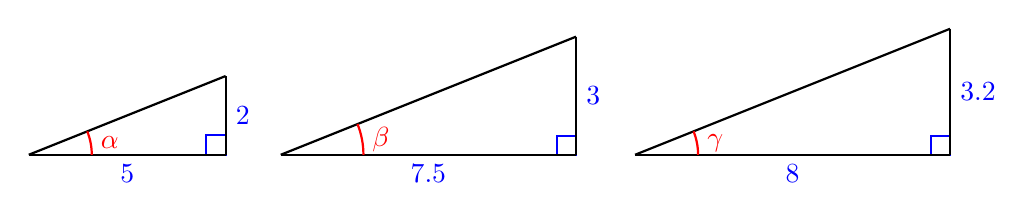
\begin{tikzpicture} 

\coordinate(A) at (0,0);
\coordinate (B) at (2.5,0 );
\coordinate (C) at (2.5,1);

\draw[blue,thick] (B) rectangle +(-0.25,0.25);
\draw[black,thick] (A)--(B) node [below,midway] {\color{blue}$5$};
\draw[black,thick] (C)--(B) node [right,midway] {\color{blue}$2$};
\draw[black,thick] (A)--(C);
\draw[red,thick] (0.8,0) arc (0:{atan(2/5)}:0.8) node[ right, midway] {$\alpha$};

\draw[blue,thick, xshift=3.2cm, scale=1.5] (2.5,0) rectangle +(-0.16,0.16);
\draw[black,thick, xshift=3.2cm, scale=1.5] (0,0)--(2.5,0) node [below,midway] {\color{blue}$7.5$};
\draw[black,thick, xshift=3.2cm, scale=1.5] (2.5,1)--(2.5,0) node [right,midway] {\color{blue}$3$};
\draw[black,thick, xshift=3.2cm, scale=1.5] (0,0)--(2.5,1);
\draw[red,thick, xshift=3.2cm, scale=1.5] (0.7,0) arc (0:{atan(2/5)}:0.7) node[ right, midway] {$\beta$};

\draw[blue,thick, xshift=7.7cm, scale=1.6] (2.5,0) rectangle +(-0.15,0.15);
\draw[black,thick, xshift=7.7cm, scale=1.6] (0,0)--(2.5,0) node [below,midway] {\color{blue}$8$};
\draw[black,thick, xshift=7.7cm, scale=1.6] (2.5,1)--(2.5,0) node [right,midway] {\color{blue}$3.2$};
\draw[black,thick, xshift=7.7cm, scale=1.6] (0,0)--(2.5,1);
\draw[red,thick, xshift=7.7cm, scale=1.6] (0.5,0) arc (0:{atan(2/5)}:0.5) node[ right, midway] {$\gamma$};

\end{tikzpicture}
\newline


Similar triangles d
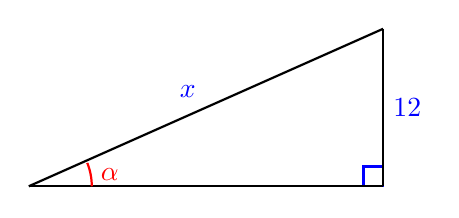
\begin{tikzpicture} 

\coordinate(A) at (0,0);
\coordinate (B) at (4.5,0 );
\coordinate (C) at (4.5,2);

\draw[blue,thick] (B) rectangle +(-0.25,0.25);
\draw[black,thick] (A)--(B);
\draw[black,thick] (C)--(B) node [right,midway] {\color{blue}$12$};
\draw[black,thick] (A)--(C) node [above left,midway] {\color{blue}$x$};
\draw[red,thick] (0.8,0) arc (0:{atan(2/5)}:0.8) node[ right, midway] {$\alpha$};

\end{tikzpicture}
\newline


Similar triangles 2
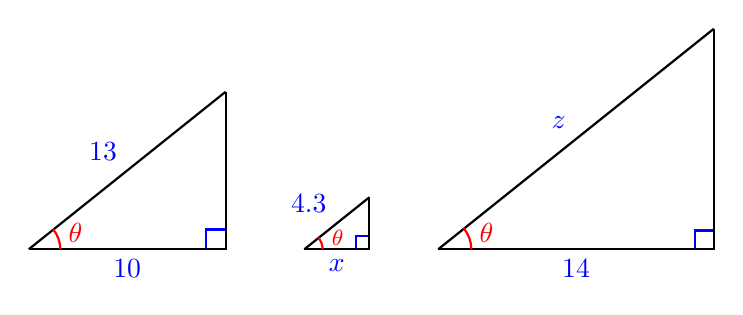
\begin{tikzpicture} 

\coordinate(A) at (0,0);
\coordinate (B) at (2.5,0 );
\coordinate (C) at (2.5,2);

\draw[blue,thick] (B) rectangle +(-0.25,0.25);
\draw[black,thick] (A)--(B) node [below,midway] {\color{blue}$10$};
\draw[black,thick] (C)--(B);
\draw[black,thick] (A)--(C) node [above left,midway] {\color{blue}$13$};
\draw[red,thick] (0.4,0) arc (0:{acos(10/13)}:0.4) node[ right, midway, yshift=2] {$\theta$};

\draw[blue,thick, xshift=3.5cm, scale=0.33] (2.5,0) rectangle +(-0.5,0.5);
\draw[black,thick, xshift=3.5cm, scale=0.33] (0,0)--(2.5,0) node [below,midway] {\color{blue}$x$};
\draw[black,thick, xshift=3.5cm, scale=0.33] (2.5,2)--(2.5,0);
\draw[black,thick, xshift=3.5cm, scale=0.33] (0,0)--(2.5,2) node [above left,midway] {\color{blue}$4.3$};
\draw[red,thick, xshift=3.5cm, scale=0.33] (0.7,0) arc (0:{acos(10/13)}:0.7) node[ right, midway, yshift=2] {\footnotesize$\theta$};


\draw[blue,thick, xshift=5.2cm, scale=1.4] (2.5,0) rectangle +(-0.17,0.17);
\draw[black,thick, xshift=5.2cm, scale=1.4] (0,0)--(2.5,0) node [below,midway] {\color{blue}$14$};
\draw[black,thick, xshift=5.2cm, scale=1.4] (2.5,2)--(2.5,0);
\draw[black,thick, xshift=5.2cm, scale=1.4] (0,0)--(2.5,2) node [above left,midway] {\color{blue}$z$};
\draw[red,thick, xshift=5.2cm, scale=1.4] (0.3,0) arc (0:{acos(10/13)}:0.3) node[ right, midway, yshift=2] {$\theta$};

\end{tikzpicture}
\newline


Similar triangles 3
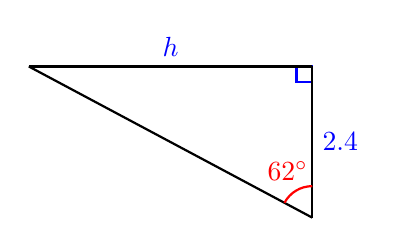
\begin{tikzpicture} [scale=.8]

\coordinate(A) at (0,0);
\coordinate (B) at (4.5,0 );
\coordinate (C) at (4.5,-2.4);

\draw[blue,thick] (B) rectangle +(-0.25,-0.25);
\draw[black,thick] (A)--(B) node [above,midway] {\color{blue}$h$};
\draw[black,thick] (C)--(B) node [right,midway] {\color{blue}$2.4$};
\draw[black,thick] (A)--(C);
\draw[red,thick] (4.5,-1.9) arc (90:152:0.5) node[ above , midway, xshift=-3] {$62\degree$};

\end{tikzpicture}
\newline


Similar triangles 3b
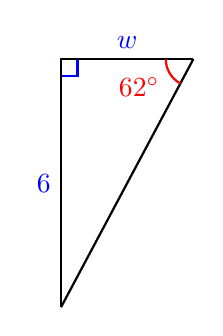
\begin{tikzpicture} [scale=.7, rotate=90]

\coordinate(A) at (0,0);
\coordinate (B) at (4.5,0 );
\coordinate (C) at (4.5,-2.4);

\draw[blue,thick] (B) rectangle +(-0.3,-0.3);
\draw[black,thick] (A)--(B) node [left,midway] {\color{blue}$6$};
\draw[black,thick] (C)--(B) node [above,midway] {\color{blue}$w$};
\draw[black,thick] (A)--(C);
\draw[red,thick] (4.5,-1.9) arc (90:152:0.5) node[ left , midway, yshift=-5] {$62\degree$};

\end{tikzpicture}
\newline


Similar triangles 3bii
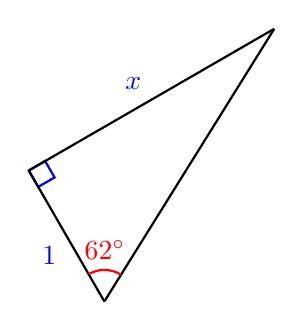
\begin{tikzpicture} [scale=.8, rotate=30]

\coordinate(A) at (0,0);
\coordinate (B) at (-4.5,0 );
\coordinate (C) at (-4.5,-2.4);

\draw[blue,thick] (B) rectangle +(0.3,-0.3);
\draw[black,thick] (A)--(B) node [above left,midway] {\color{blue}$x$};
\draw[black,thick] (C)--(B) node [below left,midway] {\color{blue}$1$};
\draw[black,thick] (A)--(C);
\draw[red,thick] (-4.5,-1.9) arc (90:28:0.5) node[ above , midway, yshift=0] {$62\degree$};

\end{tikzpicture}
\newline


\section{2.1 Side and Angle Relationships}
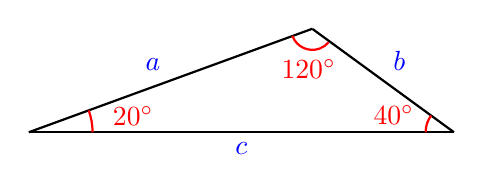
\begin{tikzpicture} [scale=.9]

\coordinate(A) at (0,0);
\coordinate (B) at (6,0 );
\coordinate (C) at (4,1.46);

\draw[black,thick] (A)--(B) node [below,midway] {\color{blue}$c$};
\draw[black,thick] (C)--(B) node [above right,midway] {\color{blue}$b$};
\draw[black,thick] (A)--(C) node [above left,midway] {\color{blue}$a$};
\draw[red,thick] (.9,0) arc (0:20:0.9) node[ right , midway, xshift=4, yshift=2] {$20\degree$};
\draw[red,thick] (5.6,0) arc (180:{180-atan(1.46/2)}:0.4) node[ left , midway, xshift=-1, yshift=3] {$40\degree$};
\draw[red,thick] (3.72,1.36) arc (200:320:0.3) node[ below , midway, yshift=0] {$120\degree$};

\end{tikzpicture}
\newline


second triangle
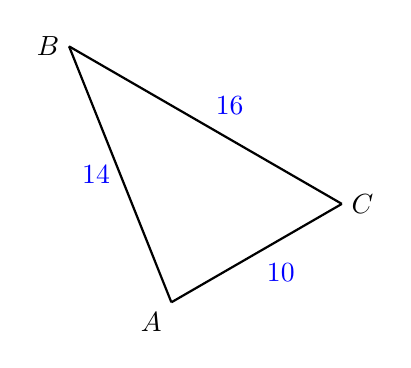
\begin{tikzpicture} [scale=.25,rotate=30]

\coordinate(A) at (0,0);
\coordinate (B) at (2,13.86 );
\coordinate (C) at (10,0);

\draw[black,thick] (A)--(B) node [left,midway] {\color{blue}$14$};
\draw[black,thick] (C)--(B) node [above right,midway] {\color{blue}$16$};
\draw[black,thick] (A)--(C) node [below right,midway] {\color{blue}$10$};

\node at (A) [anchor=north east] {$A$};
\node at (B) [anchor= east] {$B$};
\node at (C) [anchor=west] {$C$};

\end{tikzpicture}
\newline


third triangle
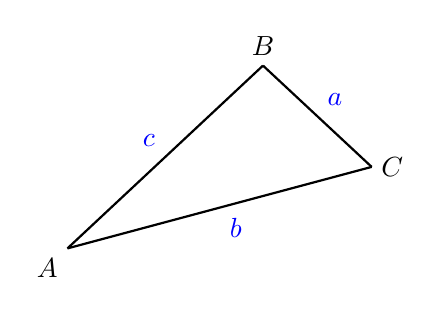
\begin{tikzpicture} [rotate=15]

\coordinate(A) at (0,0);
\coordinate (B) at (3,1.6 );
\coordinate (C) at (4,0);

\draw[black,thick] (A)--(B) node [above left,midway] {\color{blue}$c$};
\draw[black,thick] (C)--(B) node [above right,midway] {\color{blue}$a$};
\draw[black,thick] (A)--(C) node [below right,midway] {\color{blue}$b$};

\node at (A) [anchor=north east] {$A$};
\node at (B) [anchor= south] {$B$};
\node at (C) [anchor=west] {$C$};

\end{tikzpicture}
\newline


triangle inequality
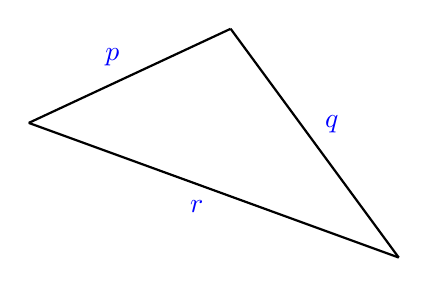
\begin{tikzpicture} [rotate=-20]

\coordinate(A) at (0,0);
\coordinate (B) at (5,0 );
\coordinate (C) at (2,2);

\draw[black,thick] (A)--(B) node [below left,midway] {\color{blue}$r$};
\draw[black,thick] (C)--(B) node [above right,midway] {\color{blue}$q$};
\draw[black,thick] (A)--(C) node [above left,midway] {\color{blue}$p$};

\end{tikzpicture}
\newline


Example 2
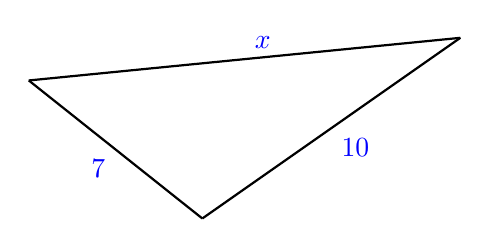
\begin{tikzpicture} [rotate=35]

\coordinate(A) at (0,0);
\coordinate (B) at (4.,0 );
\coordinate (C) at (-.8,2.7);

\draw[black,thick] (A)--(B) node [below right,midway] {\color{blue}$10$};
\draw[black,thick] (C)--(B) node [above right,midway] {\color{blue}$x$};
\draw[black,thick] (A)--(C) node [below left,midway] {\color{blue}$7$};

\end{tikzpicture}
\newline
Pythagorean Theorem triangle is in intro algebra

Example 3 picture of ladder is also in intro algebra

Example 4
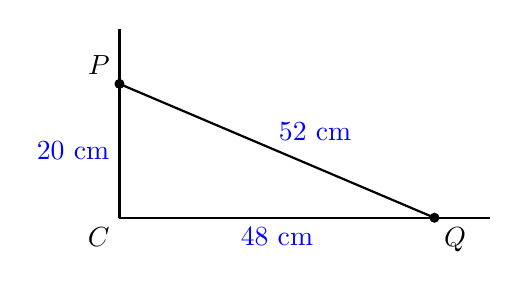
\begin{tikzpicture} 

\coordinate(A) at (0,0);
\coordinate (B) at (4,0 );
\coordinate (C) at (0,1.7);

\draw[black,thick] (A)--(B) node [below,midway] {\color{blue}$48$ cm};
\draw[black,thick] (C)--(B) node [above right,midway, xshift=-3] {\color{blue}$52$ cm};
\draw[black,thick] (A)--(C) node [left,midway] {\color{blue}$20$ cm};
\draw[black,thick] (C) -- +(0,.7);
\draw[black,thick] (B) -- +(.7,0);

\filldraw[black] (A) circle (.2pt) node[anchor=north east] {$C$};
\filldraw[black] (B) circle (1.6pt) node[anchor=north west] {$Q$};
\filldraw[black] (C) circle (1.6pt) node[anchor=south east] {$P$};

\end{tikzpicture}
\newline


hp-2.1.1
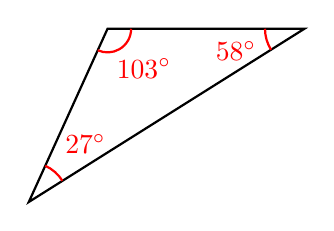
\begin{tikzpicture} 

\coordinate(A) at (0,0);
\coordinate (B) at (2.5,0 );
\coordinate (C) at (-1,-2.2);

\draw[black,thick] (A)--(B)--(C)--cycle;

\draw[red,thick] (0.3,0) arc(0:{-180+atan(2.2)}: 0.3) node[below right, midway, xshift=-5] {$103\degree$};
\draw[red,thick] (2.,0) arc(180:{180+atan(2.2/3.5)}: 0.5) node[below left, midway, yshift=3] {$58\degree$};
\draw[red,thick] (-.79,-1.74) arc({atan(2.2)}:{atan(2.2/3.5)}: 0.5) node[above right, midway, yshift=3] {$27\degree$};

\end{tikzpicture}
\newline


hp-2.1.2
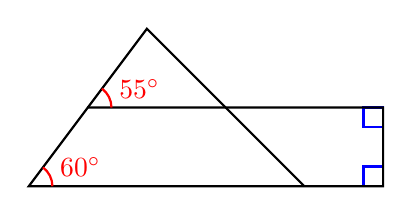
\begin{tikzpicture} 

\coordinate(A) at (0,0);
\coordinate (B) at (4.5,0 );
\coordinate (C) at (3.5,0);
\coordinate (D) at (1.5,2);
\coordinate (E) at (.75,1);
\coordinate (F) at (4.5,1);

\draw[blue,thick] (B) rectangle +(-0.25, 0.25);
\draw[blue,thick] (F) rectangle +(-0.25, -0.25);

\draw[black,thick] (A)--(B)--(F)--(E)--cycle;
\draw[black,thick] (C)--(D)--(E);

\draw[red,thick] (0.3,0) arc(0:{atan(2/1.5)}: 0.3) node[right, midway, yshift=3] {$60\degree$};
\draw[red,thick] (1.05,1) arc(0:{atan(2/1.5)}: 0.3) node[right, midway, yshift=3] {$55\degree$};

\end{tikzpicture}
\newline


hp-2.1.3
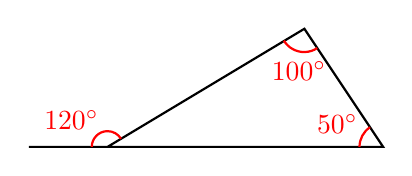
\begin{tikzpicture} 

\coordinate(A) at (0,0);
\coordinate (B) at (3.5,0 );
\coordinate (C) at (2.5,1.5);
\coordinate (D) at (-1,0);

\draw[black,thick] (A)--(B)--(C)--(A)--(D);

\draw[red,thick] (-.2,0) arc(180:{atan(1.5/2.5)}: 0.2) node[above left, midway, xshift=2, yshift=-3] {$120\degree$};
\draw[red,thick] (2.24,1.35) arc({180+atan(.6)}:{360-atan(1.5)}: 0.3) node[below , midway, xshift=0] {$100\degree$};
\draw[red,thick] (3.2,0) arc(180:{180-atan(1.5)}: 0.3) node[above left, midway, xshift=2, yshift=-3] {$50\degree$};

\end{tikzpicture}
\newline

hp-2.1.4
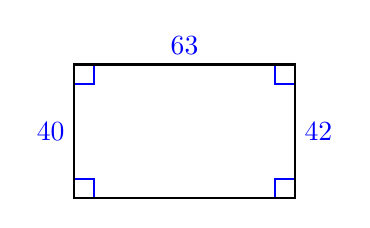
\begin{tikzpicture} 

\coordinate(A) at (0,0);
\coordinate (B) at (2.8,0 );
\coordinate (C) at (2.8,1.7);
\coordinate (D) at (0,1.7);

\draw[blue,thick] (A) rectangle +(0.25,0.25);
\draw[blue,thick] (B) rectangle +(-0.25,0.25);
\draw[blue,thick] (C) rectangle +(-0.25,-0.25);
\draw[blue,thick] (D) rectangle +(0.25,-0.25);
\draw[black,thick] (A)--(B)--(C)--(D)--cycle;

\node at (2.8,.85) [anchor = west] {\color{blue}$42$};
\node at (1.4,1.7) [anchor = south] {\color{blue}$63$};
\node at (0,.85) [anchor = east] {\color{blue}$40$};

\end{tikzpicture}
\newline

hp-2.1.5
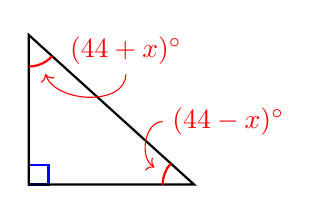
\begin{tikzpicture} 

\coordinate(A) at (0,0);
\coordinate (B) at (2.1,0 );
\coordinate (C) at (0,1.9);

\draw[blue,thick] (A) rectangle +(0.25,0.25);
\draw[black,thick] (A)--(B)--(C)--cycle;

\draw[red,thick] (0,1.5) arc(270:{360-atan(1.9/2.1)}:0.4) node[midway, xshift=0] (measure) {};
\node[anchor=north west] at (.4,2) (description) {\color{red}$(44+x)\degree$};
\draw[red,->] (description) edge[out=270,in=290,->] (measure);

\draw[red,thick] (1.7,0) arc(180:{180-atan(1.9/2.1)}:0.4) node[midway, xshift=0] (measure2) {};
\node[anchor=south west] at (1.7,0.5) (description2) {\color{red}$(44-x)\degree$};
\draw[red,->] (description2) edge[out=180,in=150,->] (measure2);
\end{tikzpicture}
\newline

hp-2.1.6
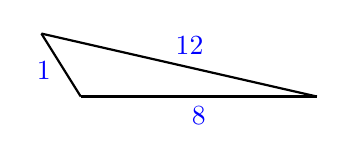
\begin{tikzpicture} 

\coordinate(A) at (0,0);
\coordinate (B) at (3,0 );
\coordinate (C) at (-.5,.8);

\draw[black,thick] (A)--(B) node[below,midway] {\color{blue}$8$};
\draw[black,thick]  (B)--(C) node[above right,midway, xshift=-5] {\color{blue}$12$};
\draw[black,thick] (A)--(C) node[ left,midway, yshift=-2] {\color{blue}$1$};

\end{tikzpicture}
\newline

hp-2.1.7
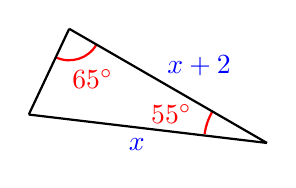
\begin{tikzpicture}  [rotate=150]

\coordinate(A) at (0,0);
\coordinate (B) at (2.9,0 );
\coordinate (C) at (2.8,1.2);

\draw[red,thick] (0.8,0) arc(0:{atan(1/2.5)}:0.8) node[above left, midway, xshift=-2, yshift=-4] {$55\degree$};
\draw[red,thick] (2.5,0) arc(180:{180-atan(12)}:0.4) node[below right, midway, xshift=-6] {$65\degree$};
\draw[black,thick] (A)--(B) node[above right,midway, xshift=-4] {\color{blue}$x+2$};
\draw[black,thick]  (B)--(C) ;
\draw[black,thick] (A)--(C) node[ below,midway, xshift=-4] {\color{blue}$x$};

\end{tikzpicture}
\newline

hp-2.1.8
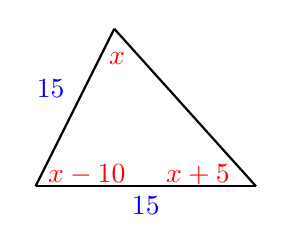
\begin{tikzpicture}  

\coordinate(A) at (0,0);
\coordinate (B) at (2.8,0 );
\coordinate (C) at (1.,2.);

\node at (A) [anchor=south west, xshift=1, yshift=-3] {\color{red}$x-10$};
\node at (B) [anchor=south east, xshift=-6, yshift=-3] {\color{red}$x+5$};
\node at (C) [anchor=north, xshift=1, yshift=-5] {\color{red}$x$};
\draw[black,thick] (A)--(B) node[below,midway] {\color{blue}$15$};
\draw[black,thick]  (B)--(C) ;
\draw[black,thick] (A)--(C) node[ above left,midway, xshift=0] {\color{blue}$15$};

\end{tikzpicture}
\newline

hp-2.1.9
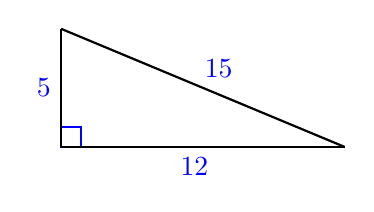
\begin{tikzpicture}  

\coordinate(A) at (0,0);
\coordinate (B) at (3.6,0 );
\coordinate (C) at (0,1.5);

\draw[blue,thick] (A) rectangle +(0.25,0.25);
\draw[black,thick] (A)--(B) node[below,midway, xshift=-3] {\color{blue}$12$};
\draw[black,thick]  (B)--(C) node[above right,midway, xshift=-3] {\color{blue}$15$};
\draw[black,thick] (A)--(C) node[left,midway, xshift=0] {\color{blue}$5$};

\end{tikzpicture}
\newline

hp-2.1.10
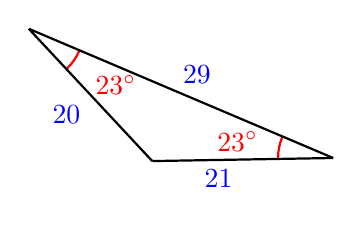
\begin{tikzpicture}  [rotate=157]

\coordinate(A) at (0,0);
\coordinate (B) at (4.2,0 );
\coordinate (C) at (2.1,0.933844);

\draw[red,thick] (.7,0) arc (0:23:.7) node [left, midway, xshift=-4, yshift=2] {$23\degree$};
\draw[red,thick] (3.5,0) arc (180:157:.7) node [below right, midway, xshift=4, yshift=-2] {$23\degree$};
\draw[black,thick] (A)--(B) node[above right,midway, xshift=-3] {\color{blue}$29$};
\draw[black,thick]  (B)--(C) node[below left,midway, xshift=0] {\color{blue}$20$};
\draw[black,thick] (A)--(C) node[below left,midway, xshift=0] {\color{blue}$21$};

\end{tikzpicture}
\newline


hp-2.1.11
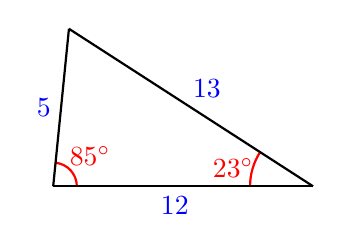
\begin{tikzpicture} 

\coordinate(A) at (0,0);
\coordinate (B) at (3.3,0 );
\coordinate (C) at (0.2,2.);

\draw[red,thick] (.3,0) arc (0:{atan(11.25)}:.3) node [above right, midway, xshift=-4, yshift=-2] {$85\degree$};
\draw[red,thick] (2.5,0) arc (180:{180-atan(2/3.1)}:.8) node [left, midway, xshift=4, yshift=0] {$23\degree$};
\draw[black,thick] (A)--(B) node[below,midway, xshift=-3] {\color{blue}$12$};
\draw[black,thick]  (B)--(C) node[above right,midway, xshift=-3] {\color{blue}$13$};
\draw[black,thick] (A)--(C) node[left,midway, xshift=0] {\color{blue}$5$};

\end{tikzpicture}
\newline


hp-2.1.12
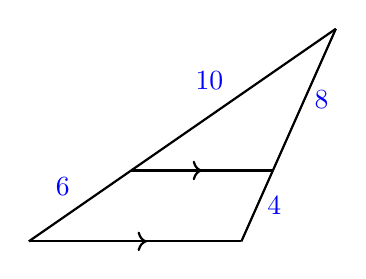
\begin{tikzpicture} 

\coordinate(A) at (0,0);
\coordinate (B) at (2.7,0 );
\coordinate (C) at (3.1,0.9);
\coordinate (D) at (3.9,2.7);
\coordinate (E) at (1.3,0.9);

\draw[black,thick] (A)--(B) ;
\draw[black,thick]  (B)--(C) node[ right,midway] {\color{blue}$4$};
\draw[black,thick] (D)--(C) node[right,midway] {\color{blue}$8$};
\draw[black,thick] (D)--(E) node[above left,midway] {\color{blue}$10$};
\draw[black,thick] (A)--(E) node[above left,midway] {\color{blue}$6$};
\draw[black,thick] (E)--(C);
\draw[black,thick, ->] (E)-- +(0.9,0);
\draw[black,thick, ->] (A)-- +(1.5,0);

\end{tikzpicture}
\newline


hp-2.1.21
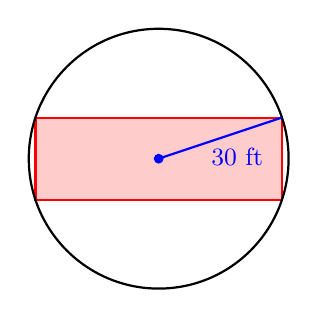
\begin{tikzpicture} [scale=.055]

\coordinate(O) at (0,0);
\coordinate(A) at (28.46,9.4868);
\coordinate (B) at (-28.46,9.4868 );
\coordinate (C) at (-28.46,-9.4868);
\coordinate (D) at (28.46,-9.4868);

\draw[fill=white!80!red,draw=red,thick] (A)--(B) --(C)--(D)--cycle;
\draw[black,thick] (O) circle (30);
\draw[blue,thick] (O) -- (A) node[below right, midway, xshift=-7] {\small 30 ft};
\filldraw [blue] (O) circle (1cm);

\end{tikzpicture}
\newline


hp-2.1.22
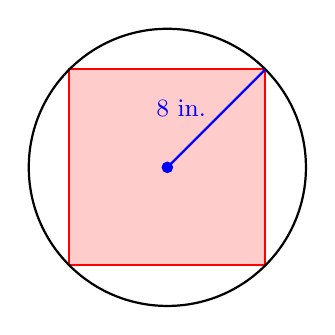
\begin{tikzpicture} [scale=.22]

\coordinate(O) at (0,0);
\coordinate(A) at (5.6569,5.6569);
\coordinate (B) at (-5.6569,5.6569);
\coordinate (C) at (-5.6569,-5.6569);
\coordinate (D) at (5.6569,-5.6569);

\draw[fill=white!80!red,draw=red,thick] (A)--(B) --(C)--(D)--cycle;
\draw[black,thick] (O) circle (8);
\draw[blue,thick] (O) -- (A) node[above left, midway, yshift=-3] {\small 8 in.};
\filldraw [blue] (O) circle (.3cm);

\end{tikzpicture}
\newline


hp-2.1.23
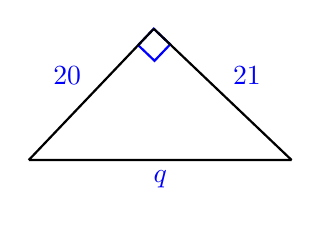
\begin{tikzpicture} [scale=.115, rotate=-133.6]

\coordinate(O) at (0,0);
\coordinate(A) at (20,0);
\coordinate (B) at (0,21);

\draw[blue,thick] (O) rectangle +(2.5,2.5);
\draw[black,thick] (O) --(A) node[above left,midway] {\color{blue}$20$};
\draw[black,thick] (B) --(A) node[below,midway] {\color{blue}$q$};
\draw[black,thick] (B) --(O) node[above right,midway] {\color{blue}$21$};

\end{tikzpicture}
\newline


hp-2.1.24
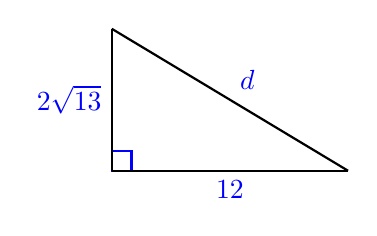
\begin{tikzpicture} [scale=.25]

\coordinate(O) at (0,0);
\coordinate(A) at (12,0);
\coordinate (B) at (0,7.2111);

\draw[blue,thick] (O) rectangle +(1,1);
\draw[black,thick] (O) --(A) node[below,midway] {\color{blue}$12$};
\draw[black,thick] (B) --(A) node[above right,midway] {\color{blue}$d$};
\draw[black,thick] (B) --(O) node[left,midway] {\color{blue}$2\sqrt{13}$};

\end{tikzpicture}
\newline


hp-2.1.25
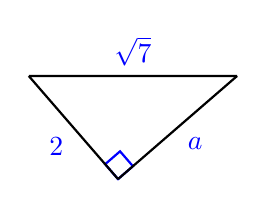
\begin{tikzpicture} [rotate=40.8934]

\coordinate(O) at (0,0);
\coordinate(A) at (2,0);
\coordinate (B) at (0,1.732);

\draw[blue,thick] (O) rectangle +(.25,.25);
\draw[black,thick] (O) --(A) node[below right,midway] {\color{blue}$a$};
\draw[black,thick] (B) --(A) node[above,midway] {\color{blue}$\sqrt{7}$};
\draw[black,thick] (B) --(O) node[below left,midway] {\color{blue}$2$};

\end{tikzpicture}
\newline


hp-2.1.26
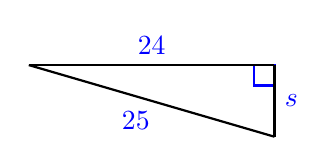
\begin{tikzpicture} [scale=.13]

\coordinate(O) at (0,0);
\coordinate(A) at (-24,0);
\coordinate (B) at (0,-7);

\draw[blue,thick] (O) rectangle +(-2.,-2.);
\draw[black,thick] (O) --(A) node[above,midway] {\color{blue}$24$};
\draw[black,thick] (B) --(A) node[below left,midway, xshift=3] {\color{blue}$25$};
\draw[black,thick] (B) --(O) node[right,midway] {\color{blue}$s$};

\end{tikzpicture}
\newline


hp-2.1.35
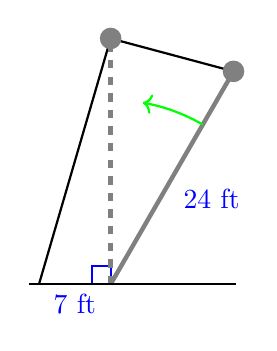
\begin{tikzpicture} [scale=.13]

\coordinate(O) at (0,0);
\coordinate(A) at (12,020.7846);
\coordinate (B) at (0,24);
\coordinate (C) at (-7,0);

\draw[blue,thick] (O) rectangle +(-1.8,1.8);
\draw[gray,ultra thick] (O) --(A) node[below right,midway] {\color{blue}24 ft};
\draw[black,thick] (B) --(A) ;
\draw[black,thick] (B) --(C);
\draw[black,thick] (O) --(C) node[below,midway] {\color{blue}7 ft};
\draw[gray,ultra thick, dashed] (O) -- (B);
\filldraw[gray] (A) circle (1cm);
\filldraw[gray] (B) circle (1 cm);
\draw[green, thick, ->] (9,15.588) arc (60:80:18);
\draw[black,thick] (-8,0) -- +(20.2,0);

\end{tikzpicture}
\newline


hp-2.1.36
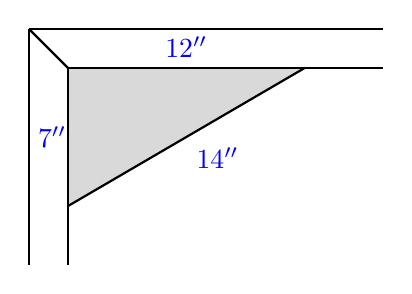
\begin{tikzpicture} [scale=.25]

\coordinate(O) at (0,0);
\coordinate(A) at (12,0);
\coordinate (B) at (0,-7);
\coordinate (C) at (-2,2);

\filldraw[gray!30!white] (O)--(A)--(B)--cycle;
\draw[black,thick] (O) --(A) node[above,midway] {\color{blue}$12^{\prime\prime }$};
\draw[black,thick] (B) --(A) node[below right,midway] {\color{blue}$14^{\prime\prime}$} ;
\draw[black,thick] (B) --(O)node[left,midway, xshift=3] {\color{blue}$7^{\prime\prime} $};
\draw[black,thick] (O) --(C) ;
\draw[black,thick] (C) -- +(0,-12);
\draw[black,thick] (B) -- +(0,-3);
\draw[black,thick] (C) -- +(18,0) ;
\draw[black,thick] (A) -- +(4,0);

\end{tikzpicture}
\newline


hp-2.1.37
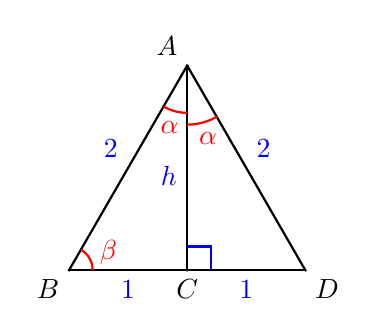
\begin{tikzpicture}  [scale=1.5]

\coordinate (B) at (0,0);
\coordinate (D) at (2,0);
\coordinate (A) at (1,1.732);
\coordinate (C) at (1,0);
\filldraw[black] (B) circle (.2pt) node[anchor=north east] {$B$};
\filldraw[black] (A) circle (.2pt) node[anchor=south east] {$A$};
\filldraw[black] (C) circle (.2pt) node[anchor=north ] {$C$};
\filldraw[black] (D) circle (.2pt) node[anchor=north west] {$D$};

\draw[blue,thick] (C) rectangle +(0.2,0.2);
\draw[black,thick] (D) --(A) node[above right,midway] {\color{blue}$2$};
\draw[black,thick] (B) --(A) node[above left,midway] {\color{blue}$2$};
\draw[black,thick] (C) --(A) node[left,midway, yshift=-3] {\color{blue}$h$} ;
\draw[black,thick] (B) --(C) node[below,midway] {\color{blue}$1 $};
\draw[black,thick] (D) --(C) node[below,midway] {\color{blue}$1 $};

\draw[red,thick] (0.2,0) arc(0:60:.2) node[ right, midway, yshift=2] {$\beta$};
\draw[red,thick] (1,1.332) arc(270:240:.4) node[ below, midway, xshift=-2] {$\alpha$};
\draw[red,thick] (1,1.232) arc(270:300:.5) node[ below, midway, xshift=2] {$\alpha$};

\end{tikzpicture}
\newline


hp-2.1.38
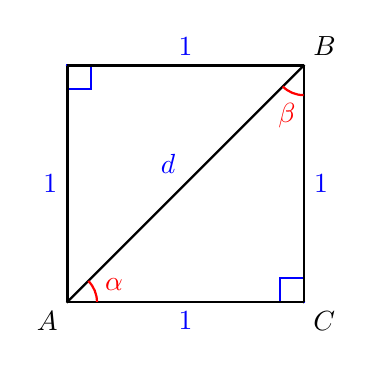
\begin{tikzpicture}  [scale=1.5]

\coordinate (A) at (0,0);
\coordinate (B) at (2,2);
\coordinate (C) at (2,0);
\coordinate (D) at (0,2);
\filldraw[black] (B) circle (.2pt) node[anchor=south west] {$B$};
\filldraw[black] (A) circle (.2pt) node[anchor=north east] {$A$};
\filldraw[black] (C) circle (.2pt) node[anchor=north west] {$C$};
\filldraw[black] (D) circle (.2pt);

\draw[blue,thick] (D) rectangle +(0.2,-0.2);
\draw[blue,thick] (C) rectangle +(-0.2,0.2);
\draw[black,thick] (D) --(A) node[left,midway] {\color{blue}$1$};
\draw[black,thick] (B) --(A) node[above left,midway] {\color{blue}$d$};
\draw[black,thick] (C) --(A) node[below,midway] {\color{blue}$1$} ;
\draw[black,thick] (B) --(C) node[right,midway] {\color{blue}$1 $};
\draw[black,thick] (B) --(D) node[above,midway] {\color{blue}$1 $};

\draw[red,thick] (0.25,0) arc(0:45:.25) node[ right, midway, yshift=2] {$\alpha$};
\draw[red,thick] (2,1.75) arc(270:225:.25) node[ below, midway, xshift=-2] {$\beta$};

\end{tikzpicture}
\newline


hp-2.1.39
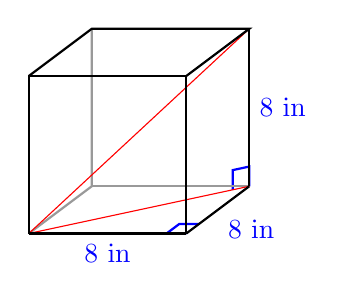
\begin{tikzpicture}  [scale=1.0]

\coordinate (A) at (0,0);
\coordinate (B) at (2,0);
\coordinate (C) at (2,2);
\coordinate (D) at (0,2);
\coordinate (E) at (.8,.6);
\coordinate (F) at (2.8,.6);
\coordinate (G) at (2.8,2.6);
\coordinate (H) at (.8,2.6);

\draw[blue,thick] (F) -- ++(0,0.25)-- ++(-.21,-.045) -- ++(0,-.25);
\draw[blue,thick] (B) -- ++(-0.25,0)-- ++(.16,.12) -- ++(.25,0);
\draw[gray!80!white,thick] (A) --(E)--(H);
\draw[gray!80!white,thick] (E)--(F);
\draw[red] (A) --(G);
\draw[red] (A) --(F);
\draw[black,thick] (B) --(F) node[below right,midway] {\color{blue}8 in};
\draw[black,thick] (F)--(G) node[ right,midway] {\color{blue}8 in};
\draw[black,thick] (B) --(A) node[below,midway] {\color{blue}8 in};
\draw[black,thick] (B)--(C)--(D) -- (A);
\draw[black,thick] (D) --(H)--(G)-- (C);

\end{tikzpicture}
\newline


hp-2.1.40
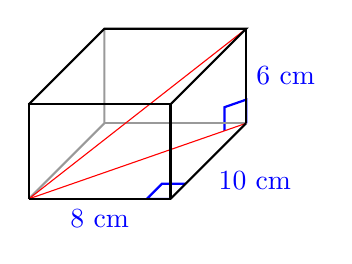
\begin{tikzpicture}  [scale=1.2]

\coordinate (A) at (0,0);
\coordinate (B) at (1.5,0);
\coordinate (C) at (1.5,1);
\coordinate (D) at (0,1);
\coordinate (E) at (.8,.8);
\coordinate (F) at (2.3,.8);
\coordinate (G) at (2.3,1.8);
\coordinate (H) at (.8,1.8);

\draw[blue,thick] (F) -- ++(0,0.25)-- ++(-.23,-.08) -- ++(0,-.25);
\draw[blue,thick] (B) -- ++(-0.25,0)-- ++(.16,.16) -- ++(.25,0);
\draw[gray!80!white,thick] (A) --(E)--(H);
\draw[gray!80!white,thick] (E)--(F);
\draw[red] (A) --(G);
\draw[red] (A) --(F);
\draw[black,thick] (B) --(F) node[below right,midway] {\color{blue}10 cm};
\draw[black,thick] (F)--(G) node[ right,midway] {\color{blue}6 cm};
\draw[black,thick] (B) --(A) node[below,midway] {\color{blue}8 cm};
\draw[black,thick] (B)--(C)--(D) -- (A);
\draw[black,thick] (D) --(H)--(G)-- (C);

\end{tikzpicture}
\newline


hp-2.1.43
\begin{tikzpicture}  [scale=1.4]

\coordinate (A) at (0,0);
\coordinate (B) at (1,0);
\coordinate (C) at (0,1);
\coordinate (D) at (0.6,0.8);

\draw[black,thick,->] (-1.4,0)--(1.4,0) node[anchor=west] {$x$};
\draw[black,thick,->] (0,-1.3)--(0,1.3) node[anchor=south] {$y$};
\draw[cyan,thick] (O) circle (1);
\draw[red,ultra thick] (-1,0)--(B)--(D)--cycle;
\filldraw[red] (D) circle (1.3pt) node[anchor=south west] {\color{blue}$(p,q)$};
\draw (1 cm,3pt) -- (1 cm,-3pt) node[anchor=north west] {$1$};
\draw (3pt,1 cm) -- (-3pt,1 cm) node[anchor=south east] {$1$};

\end{tikzpicture}
\newline


hp-2.1.44
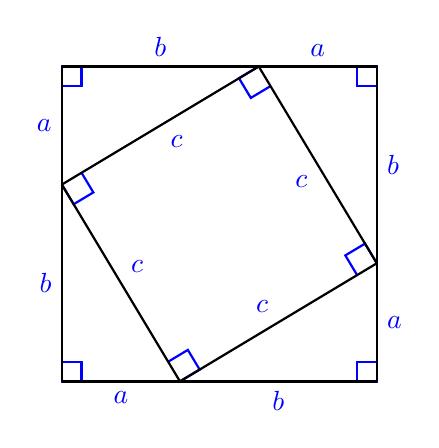
\begin{tikzpicture} 

\coordinate (A) at (0,0);
\coordinate (B) at (4,0);
\coordinate (C) at (4,4);
\coordinate (D) at (0,4);

\coordinate (E) at (1.5,0);
\coordinate (F) at (4,1.5);
\coordinate (G) at (2.5,4);
\coordinate (H) at (0,2.5);

\draw[blue,thick] (A) rectangle +(.25,.25);
\draw[blue,thick] (B) rectangle +(-.25,.25);
\draw[blue,thick] (C) rectangle +(-.25,-.25);
\draw[blue,thick] (D) rectangle +(.25,-.25);

\draw[blue,thick] (E)-- ++(.25,.15)-- ++(-.15,.25)-- ++(-.25,-.15);
\draw[blue,thick] (F)-- ++(-.15,.25)-- ++(-.25,-.15)-- ++(.15,-.25);
\draw[blue,thick] (G)-- ++(-.25,-.15)-- ++(.15,-.25)-- ++(.25,.15);
\draw[blue,thick] (H)-- ++(.15,-.25)-- ++(.25,.15)-- ++(-.15,.25);

\draw[black,thick] (A)--(E) node[below,midway] {\color{blue}$a$};
\draw[black,thick] (B)--(E) node[below,midway] {\color{blue}$b$};
\draw[black,thick] (B)--(F) node[right,midway] {\color{blue}$a$};
\draw[black,thick] (C)--(F) node[right,midway] {\color{blue}$b$};
\draw[black,thick] (C)--(G) node[above,midway] {\color{blue}$a$};
\draw[black,thick] (D)--(G) node[above,midway] {\color{blue}$b$};
\draw[black,thick] (D)--(H) node[left,midway] {\color{blue}$a$};
\draw[black,thick] (A)--(H) node[left,midway] {\color{blue}$b$};

\draw[black,thick] (H)--(E) node[above right,midway] {\color{blue}$c$};
\draw[black,thick] (F)--(E) node[above left,midway] {\color{blue}$c$};
\draw[black,thick] (F)--(G) node[below left,midway] {\color{blue}$c$};
\draw[black,thick] (H)--(G) node[below right,midway] {\color{blue}$c$};

\end{tikzpicture}
\newline

\section {2.2 Right triangle trig}

first triangle
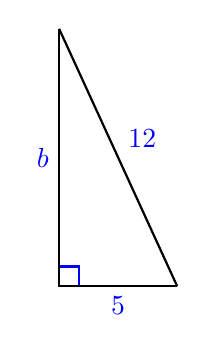
\begin{tikzpicture}  

\coordinate (A) at (0,0);
\coordinate (B) at (1.5,0);
\coordinate (C) at (0,3.27);

\draw[blue,thick] (A) rectangle +(0.25,0.25);
\draw[black,thick] (A)--(B) node[below,midway] {\color{blue}$5$};
\draw[black,thick] (A)--(C) node[left,midway] {\color{blue}$b$};
\draw[black,thick] (B)--(C) node[above right,midway] {\color{blue}$12$};

\end{tikzpicture}
\newline

second triangle
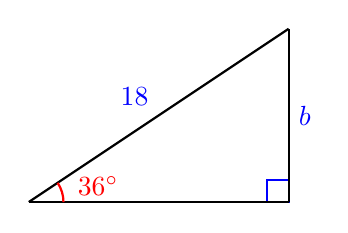
\begin{tikzpicture} [scale=1.1] 

\coordinate (A) at (0,0);
\coordinate (B) at (-3,0);
\coordinate (C) at (0,2.);

\draw[blue,thick] (A) rectangle +(-0.25,0.25);
\draw[black,thick] (A)--(B);
\draw[black,thick] (A)--(C) node[right,midway] {\color{blue}$b$};
\draw[black,thick] (B)--(C) node[above left,midway] {\color{blue}$18$};
\draw[red,thick] (-2.6,0) arc(0:{atan(2/3)}:.4) node[right,midway, xshift=2,yshift=2] {$36\degree$};

\end{tikzpicture}
\newline

overlapping triangles
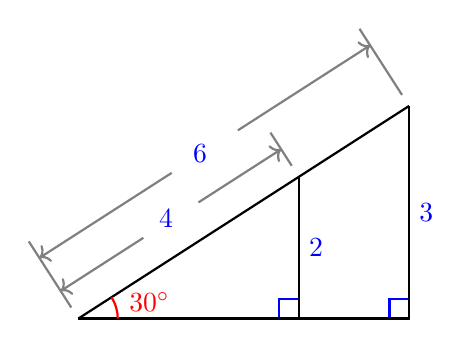
\begin{tikzpicture}

\coordinate (A) at (0,0);
\coordinate (B) at (4.2,0);
\coordinate (C) at (4.2,2.7);
\coordinate (D) at (2.8,0);
\coordinate (E) at (2.8,1.8);

\draw[blue,thick] (B) rectangle +(-0.25,0.25);
\draw[blue,thick] (D) rectangle +(-0.25,0.25);
\draw[black,thick] (D)--(E)node[right,midway] {\color{blue}$2$};
\draw[black,thick] (A)--(B);
\draw[black,thick] (A)--(C);
\draw[black,thick] (B)--(C) node[right,midway] {\color{blue}$3$};

\draw [red, thick] (0.5,0) arc(0:{atan(9/14)}:.5) node[right,midway, xshift=1, yshift=2] {$30\degree$};

\draw[gray, thick] (-.09,.14) -- ++(-.27,.42) -- ++(-.27,.42);
\draw[gray, thick] (C)++(-.09,.14) -- ++(-.27,.42) -- ++(-.27,.42);
\draw[gray, thick] (E)++(-.09,.14) -- ++(-.27,.42);
\draw[gray, thick, <-] (E)++(-.225,.35) -- ++(-1.05,-.675);
\draw[gray, thick, <-] (A)++(-.225,.35) -- ++(1.05,.675) node [above right, xshift=2] {\color{blue}$4$};
\draw[gray, thick, <-] (A)++(-.225,.35)++(-.27,.42) -- ++(1.68,1.08) node [above right, xshift=4] {\color{blue}$6$};
\draw[gray, thick, <-] (C)++(-.225,.35)++(-.27,.42) -- ++(-1.68,-1.08);

\end{tikzpicture}
\newline

definition of sine
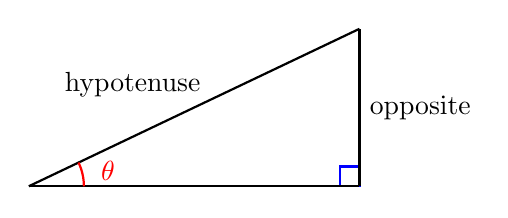
\begin{tikzpicture}

\coordinate (A) at (0,0);
\coordinate (B) at (4.2,0);
\coordinate (C) at (4.2,2);

\draw[blue,thick] (B) rectangle +(-0.25,0.25);
\draw[black,thick] (A)--(B);
\draw[black,thick] (A)--(C) node[above left,midway, xshift=6] {hypotenuse};
\draw[black,thick] (B)--(C) node[right,midway] {opposite};

\draw [red, thick] (0.7,0) arc(0:{atan(2/4.2)}:.7) node[right,midway, xshift=3, yshift=1] {$\theta$};

\end{tikzpicture}
\newline

Example 1a
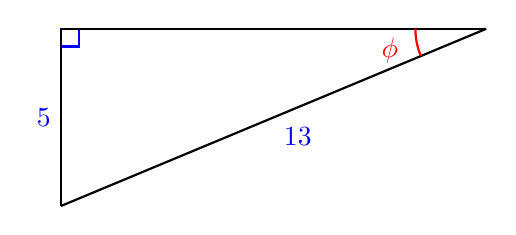
\begin{tikzpicture} [scale=.9]

\coordinate (A) at (0,0);
\coordinate (B) at (6,0);
\coordinate (C) at (0,-2.5);

\draw[blue,thick] (A) rectangle +(0.25,-0.25);
\draw[black,thick] (A)--(B);
\draw[black,thick] (A)--(C) node[left,midway] {\color{blue}5};
\draw[black,thick] (B)--(C) node[below right,midway] {\color{blue}13};

\draw [red, thick] (5,0) arc(180:{180+atan(5/12)}:1) node[left,midway, xshift=-3, yshift=-3] {$\phi$};

\end{tikzpicture}
\newline

Example 1b
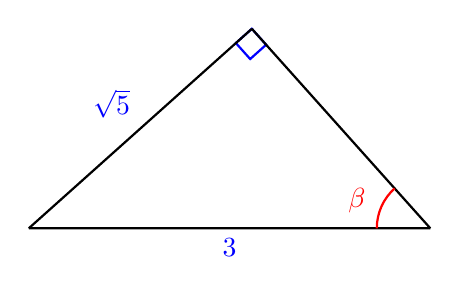
\begin{tikzpicture}  [rotate=-138.1888, scale=1.7]

\coordinate (A) at (0,0);
\coordinate (B) at (2.236,0);
\coordinate (C) at (0,2);

\draw[blue,thick] (A) rectangle +(0.16,0.16);
\draw[black,thick] (A)--(B) node[above left,midway] {\color{blue}$\sqrt{5}$};
\draw[black,thick] (A)--(C);
\draw[black,thick] (B)--(C) node[below ,midway] {\color{blue}3};

\draw [red, thick] (C)++(0,-.4) arc(-90:{-atan(2/2.236)}:.4) node[ left,midway, xshift=-2, yshift=2] {$\beta$};

\end{tikzpicture}
\newline


Exercise 1
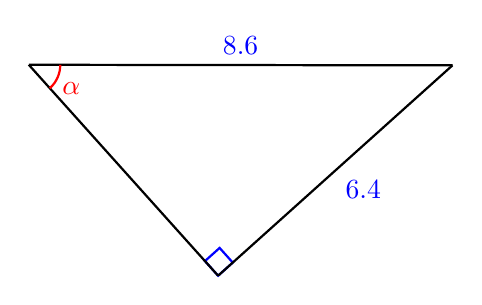
\begin{tikzpicture}  [rotate=41.91]

\coordinate (A) at (0,0);
\coordinate (B) at (4,0);
\coordinate (C) at (0,3.6);

\draw[blue,thick] (A) rectangle +(0.25,0.25);
\draw[black,thick] (A)--(B) node[below right,midway] {\color{blue}$6.4$};
\draw[black,thick] (A)--(C);
\draw[black,thick] (B)--(C) node[above ,midway] {\color{blue}8.6};

\draw [red, thick] (C)++(0,-.4) arc(-90:{-atan(0.9)}:.4) node[ below right,midway, xshift=-2, yshift=2] {$\alpha$};

\end{tikzpicture}
\newline


Caution
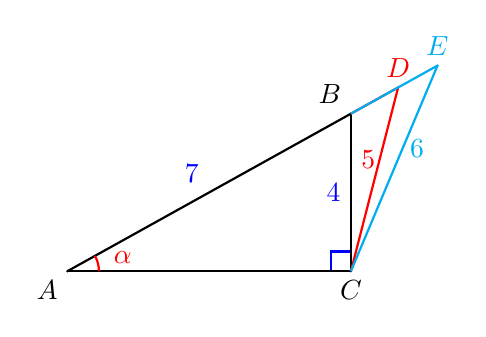
\begin{tikzpicture}  

\coordinate (A) at (0,0);
\coordinate (B) at (3.6,2);
\coordinate (C) at (3.6,0);
\coordinate (D) at (4.2,2.333);
\coordinate (E) at (4.7,2.611);

\filldraw[black] (A) circle (0.2pt) node[anchor=north east] {$A$};
\filldraw[black] (B) circle (0.2pt) node[anchor=south east] {$B$};
\filldraw[black] (C) circle (0.2pt) node[anchor=north ] {$C$};
\filldraw[red] (D) circle (0.2pt) node[anchor=south ] {\color{red}$D$};
\filldraw[cyan] (E) circle (0.2pt) node[anchor=south ] {\color{cyan}$E$};

\draw[blue,thick] (C) rectangle +(-0.25,0.25);
\draw[black,thick] (A)--(B) node[above left,midway] {\color{blue}$7$};
\draw[black,thick] (A)--(C);
\draw[black,thick] (B)--(C) node[left ,midway] {\color{blue}4};
\draw[red,thick] (D)--(C) node[left ,midway, xshift=4, yshift=7] {\color{red}5};
\draw[red,thick] (D)--(B);
\draw[cyan,thick] (E)--(C) node[right ,midway, xshift=2, yshift=7] {6};
\draw[cyan,thick] (E)--(B);

\draw [red, thick] (.4,0) arc(0:{atan(2/3.6)}:.4) node[ right,midway, xshift=2, yshift=2] {$\alpha$};

\end{tikzpicture}
\newline


compare sines
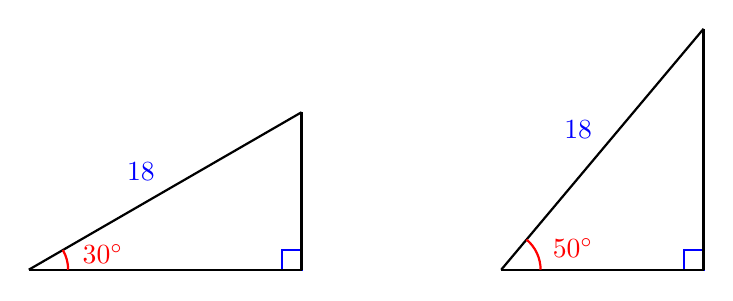
\begin{tikzpicture}  

\coordinate (A) at (0,0);
\coordinate (B) at (3.464,0);
\coordinate (C) at (3.464,2);

\draw[blue,thick] (B) rectangle +(-0.25,0.25);
\draw[black,thick] (A)--(B);
\draw[black,thick] (C)--(B);
\draw[black,thick] (A)--(C) node[above left,midway] {\color{blue}$18$};

\draw [red, thick] (.5,0) arc(0:30:.5) node[ right,midway, xshift=2, yshift=2] {$30\degree$};

\coordinate (D) at (6,0);
\coordinate (E) at (8.57,0);
\coordinate (F) at (8.57,3.06);

\draw[blue,thick] (E) rectangle +(-0.25,0.25);
\draw[black,thick] (D)--(E);
\draw[black,thick] (F)--(E);
\draw[black,thick] (D)--(F) node[above left,midway] {\color{blue}$18$};

\draw [red, thick] (D)++(.5,0) arc(0:50:.5) node[ right,midway, xshift=2, yshift=2] {$50\degree$};

\end{tikzpicture}
\newline

3 similar triangles
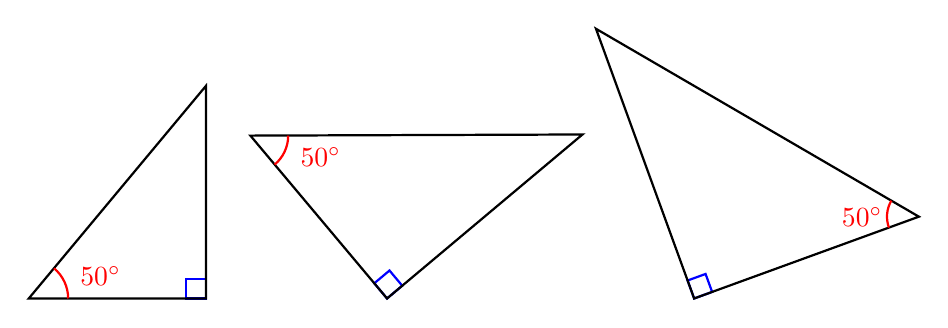
\begin{tikzpicture}  

\coordinate (A) at (0,0);
\coordinate (B) at (-2.25,0);
\coordinate (C) at (0,2.7);

\draw[blue,thick] (A) rectangle +(-0.25,0.25);
\draw[black,thick] (A)--(B) -- (C) -- cycle;
\draw [red, thick] (B)++(.5,0) arc(0:50:.5) node[ right,midway, xshift=2, yshift=2] {$50\degree$};

\draw[blue,thick,xshift=2.3cm, scale=1.2, rotate=-50] (0,0) rectangle +(-0.21,0.21);
\draw[black,thick,xshift=2.3cm, scale=1.2, rotate=-50] (0,0)--(-2.25,0) -- (0,2.7) -- cycle;
\draw [red, thick,xshift=2.3cm, scale=1.2, rotate=-50] (-2.25,0)++(.4,0) arc(0:50:.4) node[ right,midway, xshift=2, yshift=-2] {$50\degree$};


\draw[blue,thick,xshift=6.2cm, scale=1.35, rotate=20] (0,0) rectangle +(0.18,0.18);
\draw[black,thick,xshift=6.2cm, scale=1.35, rotate=20] (0,0)--(2.25,0) -- (0,2.7) -- cycle;
\draw [red, thick,xshift=6.2cm, scale=1.35, rotate=20] (2.25,0)++(-.3,0) arc(180:130:.3) node[ left,midway, xshift=2, yshift=-1] {$50\degree$};
\end{tikzpicture}
\newline

example 3
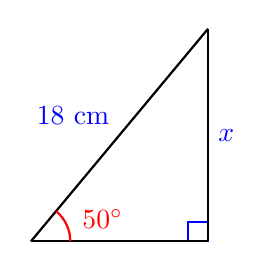
\begin{tikzpicture}  

\coordinate (A) at (0,0);
\coordinate (B) at (-2.25,0);
\coordinate (C) at (0,2.7);

\draw[blue,thick] (A) rectangle +(-0.25,0.25);
\draw[black,thick] (A)--(B);
\draw[black,thick] (A)-- (C) node[right,midway] {\color{blue}$x$};
\draw[black,thick] (B) -- (C) node[above left, midway] {\color{blue}18 cm};
\draw [red, thick] (B)++(.5,0) arc(0:50:.5) node[ right,midway, xshift=2, yshift=2] {$50\degree$};

\end{tikzpicture}
\newline

exercise 3
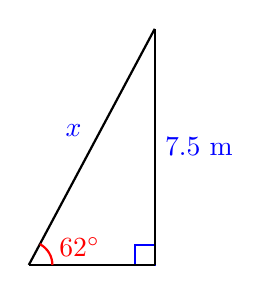
\begin{tikzpicture}  

\coordinate (A) at (0,0);
\coordinate (B) at (1.6,3);
\coordinate (C) at (1.6,0);

\draw[blue,thick] (C) rectangle +(-0.25,0.25);
\draw[black,thick] (A)--(B) node[above left,midway] {\color{blue}$x$};
\draw[black,thick] (A)-- (C) ;
\draw[black,thick] (B) -- (C) node[right, midway] {\color{blue}7.5 m};
\draw [red, thick] (A)++(.3,0) arc(0:62:.3) node[ right,midway, xshift=0, yshift=2] {$62\degree$};

\end{tikzpicture}
\newline

cliff
\begin{tikzpicture}  

\coordinate (A) at (0,0);
\coordinate (B) at (-5,0);
\coordinate (C) at (0,2.5);

\draw[blue,thick] (A) rectangle +(-0.25,0.25);
\draw[black,thick] (A)--(B) node[below,midway, xshift=17] {\color{red}angle of elevation};
\draw[black,thick] (A)-- (C)  node[right, midway] {cliff};
\draw[gray,thick, dashed] (B) -- (C);
\draw [red, thick] (B)++(.5,0) arc(0:{atan(.5)}:.5) node[right,midway, xshift=-5](angle) {};

\draw[red] (-3.4,-.3) edge[out=180,in=10,->] (angle);

\end{tikzpicture}
\newline

definition of tangent
\begin{tikzpicture}

\coordinate (A) at (0,0);
\coordinate (B) at (4.2,0);
\coordinate (C) at (4.2,2);

\draw[blue,thick] (B) rectangle +(-0.25,0.25);
\draw[black,thick] (A)--(B) node[below,midway] {adjacent};
\draw[black,thick] (A)--(C);
\draw[black,thick] (B)--(C) node[right,midway] {opposite};

\draw [red, thick] (0.7,0) arc(0:{atan(2/4.2)}:.7) node[right,midway, xshift=3, yshift=1] {$\theta$};

\end{tikzpicture}
\newline


exercise 4
\begin{tikzpicture}

\coordinate (A) at (0,0);
\coordinate (B) at (4,0);
\coordinate (C) at (4,1.84);

\draw[blue,thick] (B) rectangle +(-0.25,0.25);
\draw[black,thick] (A)--(B) node[below,midway] {\color{blue}50 ft};
\draw[black,thick] (A)--(C) node[above left,midway] {\color{blue}$c$};
\draw[black,thick] (B)--(C) node[right,midway] {\color{blue}$x$};

\draw [red, thick] (0.7,0) arc(0:24.7:.7) node[right,midway, xshift=3, yshift=2] {$24.7\degree$};

\end{tikzpicture}
\newline

definition of cosine
\begin{tikzpicture}

\coordinate (A) at (0,0);
\coordinate (B) at (4.2,0);
\coordinate (C) at (4.2,2);

\draw[blue,thick] (B) rectangle +(-0.25,0.25);
\draw[black,thick] (A)--(B) node[below,midway] {adjacent};
\draw[black,thick] (A)--(C) node[above left,midway, xshift=6] {hypotenuse};
\draw[black,thick] (B)--(C);

\draw [red, thick] (0.7,0) arc(0:{atan(2/4.2)}:.7) node[right,midway, xshift=3, yshift=1] {$\theta$};

\end{tikzpicture}
\newline

example 5
\begin{tikzpicture} [scale=.8]

\coordinate (A) at (0,0);
\coordinate (B) at (4,0);
\coordinate (C) at (0,-3);

\draw[blue,thick] (A) rectangle +(0.25,-0.25);
\draw[black,thick] (A)--(B) node[above,midway] {\color{blue}8 in};
\draw[black,thick] (A)--(C) node[left,midway] {\color{blue}6 in};
\draw[black,thick] (B)--(C);

\draw [red, thick] (0,-2.6) arc(90:{atan(.75)}:.4) node[above right,midway, xshift=-2, yshift=0] {$\theta$};

\end{tikzpicture}
\newline

20deg, 40deg, 60 deg
\begin{tikzpicture} 

\coordinate (A) at (0,0);
\coordinate (B) at (2.82,0);
\coordinate (C) at (2.82,1.03);

\draw[blue,thick] (B) rectangle +(-0.25,0.25);
\draw[black,thick] (A)--(B)--(C)--cycle;
\draw [red, thick] (.6,0) arc(0:20:.6) node[right,midway, xshift=5, yshift=2] {$20\degree$};

\draw[blue,thick] (5.4,0) rectangle +(-0.25,0.25);
\draw[black,thick] (3.1,0)--(5.4,0)--(5.4,1.93)--cycle;
\draw [red, thick] (3.6,0) arc(0:40:.5) node[right,midway, yshift=2] {$40\degree$};

\draw[blue,thick] (7.2,0) rectangle +(-0.25,0.25);
\draw[black,thick] (5.7,0)--(7.2,0)--(7.2,2.6)--cycle;
\draw [red, thick] (6.1,0) arc(0:60:.4) node[right,midway, yshift=2] {$60\degree$};

\end{tikzpicture}
\newline

trig ratios
\begin{tikzpicture}

\coordinate (A) at (0,0);
\coordinate (B) at (4.2,0);
\coordinate (C) at (4.2,2);

\draw[blue,thick] (B) rectangle +(-0.25,0.25);
\draw[black,thick] (A)--(B) node[below,midway] {adjacent};
\draw[black,thick] (A)--(C) node[above left,midway, xshift=6] {hypotenuse};
\draw[black,thick] (B)--(C) node[right,midway] {opposite};

\draw [red, thick] (0.7,0) arc(0:{atan(2/4.2)}:.7) node[right,midway, xshift=3, yshift=1] {$\theta$};

\end{tikzpicture}
\newline

example 6
\begin{tikzpicture}

\coordinate (A) at (0,0);
\coordinate (B) at (-1.17,0);
\coordinate (C) at (0,3.8);
\coordinate (D) at (1.17,0);

\draw[blue,thick] (A) rectangle +(0.25,0.25);
\draw[black,thick] (D)--(B)--(A) ;
\draw[gray,thick] (C)--(A) node[left,midway, yshift=-10] {\color{blue}$h$};
\draw[black,thick] (B)--(C) node[above left,midway, yshift=-4] {\color{blue}16 m};
\draw[black,thick] (D)--(C) node[above right,midway, yshift=-4] {\color{blue}16 m};

\draw [red, thick] (0,2.3) arc(-90:{-atan(3.8/1.17)}:1.5) node[below,midway, xshift=1, yshift=-4] {\small$17\degree$};

\end{tikzpicture}
\newline

2.1 algebraRefresh5
\begin{tikzpicture}[scale=.35]

\draw[thick,->] (-5,0) -- (7,0) node[anchor=west] {$x$};
\draw[thick,->] (0,-3) -- (0,3) node[anchor=south] {$y$};
`
\foreach \x in {-5,...,6}
    \draw (\x cm,5pt) -- (\x cm,-5pt) ;
\foreach \y in {-3,...,2}
    \draw (5pt,\y cm) -- (-5pt,\y cm)  ;

\coordinate (A) at (-5,-2);
\coordinate (B) at (5,2);
\coordinate (C) at (7,2.8);
\coordinate (O) at (0,0);

\draw[blue, thick] (A)--(C);

\filldraw[red] (B) circle (5pt) node[anchor=south east,xshift=0,yshift=0] {$(5,2)$};
\filldraw[red] (O) circle (5pt) ;

\end{tikzpicture}
\newline

2.1 algebraRefresh6
\begin{tikzpicture}[xscale=.3, yscale=0.16]

\draw[thick,->] (-9,0) -- (7,0) node[anchor=west] {$x$};
\draw[thick,->] (0,-3) -- (0,11) node[anchor=south] {$y$};
`
\foreach \x in {-9,...,6}
    \draw (\x cm,5pt) -- (\x cm,-5pt) ;
\foreach \y in {-3,...,10}
    \draw (5pt,\y cm) -- (-5pt,\y cm)  ;

\coordinate (A) at (-5,8);
\coordinate (B) at (2,-3.2);
\coordinate (C) at (-7,11.2);
\coordinate (O) at (0,0);

\draw[blue, thick] (B)--(C);

\filldraw[red] (A) ellipse (6pt and 12pt) node[anchor=north east,xshift=0,yshift=0] {$(-5,8)$};
\filldraw[red] (O) ellipse (6pt and 12pt)  ;

\end{tikzpicture}
\newline

2.1 algebraRefresh7
\begin{tikzpicture}[xscale=.3, yscale=0.2]

\draw[thick,->] (-6,0) -- (6,0) node[anchor=west] {$x$};
\draw[thick,->] (0,-6) -- (0,6) node[anchor=south] {$y$};
`
\foreach \x in {-6,...,5}
    \draw (\x cm,5pt) -- (\x cm,-5pt) ;
\foreach \y in {-6,...,5}
    \draw (5pt,\y cm) -- (-5pt,\y cm)  ;

\coordinate (A) at (-2,3);
\coordinate (B) at (-4,5.4);
\coordinate (C) at (5,-5.4);
\coordinate (O) at (3,-3);

\draw[blue, thick] (B)--(C);

\filldraw[red] (A) ellipse (6pt and 9pt) node[anchor=north east,xshift=2,yshift=2] {$(-2,3)$};
\filldraw[red] (O) ellipse (6pt and 9pt)  node[anchor=south west,xshift=-2,yshift=-5] {$(3,-3)$};

\end{tikzpicture}
\newline

2.1 algebraRefresh8
\begin{tikzpicture}[xscale=.3, yscale=0.2]

\draw[thick,->] (-6,0) -- (10,0) node[anchor=west] {$x$};
\draw[thick,->] (0,-7) -- (0,4) node[anchor=south] {$y$};

\foreach \x in {-6,...,9}
    \draw (\x cm,9pt) -- (\x cm,-9pt) ;
\foreach \y in {-7,...,3}
    \draw (5pt,\y cm) -- (-5pt,\y cm)  ;

\coordinate (A) at (-4,-5);
\coordinate (B) at (-6,-6);
\coordinate (C) at (10,2);
\coordinate (O) at (4,-1);

\draw[blue, thick] (B)--(C);

\filldraw[red] (A) ellipse (6pt and 9pt) node[anchor=north west,xshift=2,yshift=-2, fill=white] {$(-2,3)$};
\filldraw[red] (O) ellipse (6pt and 9pt)  node[anchor=north west,xshift=-5,yshift=-1] {$(3,-3)$};

\end{tikzpicture}
\newline

hmwk 2.2.1
\begin{tikzpicture}

\coordinate (A) at (0,0);
\coordinate (B) at (3,6.433);
\coordinate (C) at (3,0);
\coordinate (D) at (2,4.289);
\coordinate (E) at (2,0);

\draw[blue,thick] (C) rectangle +(-.25,.25);
\draw[blue,thick] (E) rectangle +(-.25,.25);
\draw[black, thick] (A)--(B)--(C)--cycle;
\draw[black,thick] (D)--(E);

\draw[red,thick] (0.3,0) arc(0:65:.3) node[right, midway, yshift=2] {$65\degree$};

\filldraw[black] (A) circle (.2pt) node[anchor=north east] {$A$};
\filldraw[black] (B) circle (.2pt) node[anchor=west] {$B$};
\filldraw[black] (C) circle (.2pt) node[anchor=north west] {$C$};
\filldraw[black] (D) circle (.2pt) node[anchor=south east] {$D$};
\filldraw[black] (E) circle (.2pt) node[anchor=north ] {$E$};

\end{tikzpicture}
\newline

hmwk 2.2.3
\begin{tikzpicture}

\coordinate (A) at (0,0);
\coordinate (B) at (3.5,2.9368);
\coordinate (C) at (3.5,0);
\coordinate (D) at (-2.4,-2.013);
\coordinate (E) at (-2.4,0);

\draw[blue,thick] (C) rectangle +(-.25,.25);
\draw[blue,thick] (E) rectangle +(.25,-.25);
\draw[black, thick] (B)--(C)--(E)--(D)--cycle;

\draw[red,thick] (0.4,0) arc(0:40:.4) node[right, midway, yshift=3] {$40\degree$};

\filldraw[black] (A) circle (.2pt) node[anchor=north ] {$A$};
\filldraw[black] (B) circle (.2pt) node[anchor=west] {$B$};
\filldraw[black] (C) circle (.2pt) node[anchor=north west] {$C$};
\filldraw[black] (D) circle (.2pt) node[anchor= east] {$D$};
\filldraw[black] (E) circle (.2pt) node[anchor=east ] {$E$};

\end{tikzpicture}
\newline

hmwk 2.2.5
\begin{tikzpicture}

\coordinate (A) at (0,0);
\coordinate (B) at (3,0);
\coordinate (C) at (0,-2);

\draw[blue,thick] (A) rectangle +(.25,-.25);

\draw[black, thick] (B)--(C) node[below right, midway] {\color{blue}$v$};
\draw[black, thick] (B)--(A) node[above, midway] {\color{blue}$12$};
\draw[black, thick] (A)--(C) node[left, midway] {\color{blue}$8$};

\draw[red,thick] (B)++(-0.6,0) arc(180:{180+atan(2/3)}:.6) node[left, midway, yshift=-3] {$\theta$};

\end{tikzpicture}
\newline

hmwk 2.2.6
\begin{tikzpicture} [scale=1.1]

\coordinate (A) at (0,0);
\coordinate (B) at (1,0);
\coordinate (C) at (0,2);

\draw[blue,thick] (A) rectangle +(.25,.25);

\draw[black, thick] (B)--(C) node[above right, midway] {\color{blue}$z$};
\draw[black, thick] (B)--(A) node[below, midway] {\color{blue}$5$};
\draw[black, thick] (A)--(C) node[left, midway] {\color{blue}$10$};

\draw[red,thick] (B)++(-0.3,0) arc(180:{180-atan(2)}:.3) node[left, midway, yshift=3] {$\theta$};

\end{tikzpicture}
\newline

hmwk 2.2.7
\begin{tikzpicture}

\coordinate (A) at (0,0);
\coordinate (B) at (4.2,0);
\coordinate (C) at (0,1);

\draw[blue,thick] (A) rectangle +(.25,.25);

\draw[black, thick] (B)--(C) node[above right, midway] {\color{blue}$16$};
\draw[black, thick] (B)--(A) node[below, midway] {\color{blue}$w$};
\draw[black, thick] (A)--(C) node[left, midway] {\color{blue}$4$};

\draw[red,thick] (C)++(0,-.3) arc(-90:{-atan(1/4.2)}:.3) node[below, midway, xshift=1, yshift=1] {$\theta$};

\end{tikzpicture}
\newline

hmwk 2.2.8
\begin{tikzpicture}

\coordinate (A) at (0,0);
\coordinate (B) at (-1.8,0);
\coordinate (C) at (0,2.6);

\draw[blue,thick] (A) rectangle +(-.25,.25);

\draw[black, thick] (B)--(C) node[above left, midway] {\color{blue}$24$};
\draw[black, thick] (B)--(A) node[below, midway] {\color{blue}$m$};
\draw[black, thick] (A)--(C) node[right, midway] {\color{blue}$20$};

\draw[red,thick] (C)++(0,-.5) arc(270:{180+atan(2.6/1.8)}:.5) node[below, midway, xshift=-1] {$\theta$};

\end{tikzpicture}
\newline

hmwk 2.2.9
\begin{tikzpicture}

\coordinate (A) at (0,0);
\coordinate (B) at (-3,0);
\coordinate (C) at (0,-1.2);

\draw[blue,thick] (A) rectangle +(-.25,-.25);

\draw[black, thick] (B)--(C) node[below left, midway] {\color{blue}$n$};
\draw[black, thick] (B)--(A) node[above, midway] {\color{blue}$16$};
\draw[black, thick] (A)--(C) node[right, midway] {\color{blue}$2\sqrt{3}$};

\draw[red,thick] (B)++(.9,0) arc(0:{-atan(.4)}:.9) node[right, midway, yshift=-1] {$\theta$};

\end{tikzpicture}
\newline

hmwk 2.2.10
\begin{tikzpicture}

\coordinate (A) at (0,0);
\coordinate (B) at (-3,0);
\coordinate (C) at (0,1.8);

\draw[blue,thick] (A) rectangle +(-.25,.25);

\draw[black, thick] (B)--(C) node[above left, midway] {\color{blue}$2\sqrt{5}$};
\draw[black, thick] (B)--(A) node[below, midway] {\color{blue}$\sqrt{7}$};
\draw[black, thick] (A)--(C) node[right, midway] {\color{blue}$d$};

\draw[red,thick] (C)++(0,-0.3) arc(-90:{-180+atan(.6)}:.3) node[below left, midway, xshift=1] {$\theta$};

\end{tikzpicture}
\newline

hp2-2-11ans
\begin{tikzpicture}

\coordinate (A) at (0,0);
\coordinate (B) at (1.2,1.6);
\coordinate (C) at (1.2,0);

\draw[blue,thick] (C) rectangle +(-.25,.25);

\draw[black, thick] (B)--(C) node[right, midway] {\color{blue}$4$};
\draw[black, thick] (B)--(A) node[above left, midway] {\color{blue}$5$};
\draw[black, thick] (A)--(C) node[below, midway] {\color{blue}$3$};

\draw[red,thick] (A)++(.3,0) arc(0:{atan(4/3)}:.3) node[right, midway, yshift=1] {$\theta$};

\coordinate (A) at (2,-.5);
\coordinate (B) at (4.4,2.7);
\coordinate (C) at (4.4,-.5);

\draw[blue,thick] (C) rectangle +(-.25,.25);

\draw[black, thick] (B)--(C) node[right, midway] {\color{blue}$8$};
\draw[black, thick] (B)--(A) node[above left, midway] {\color{blue}$10$};
\draw[black, thick] (A)--(C) node[below, midway] {\color{blue}$6$};

\draw[red,thick] (A)++(.3,0) arc(0:{atan(4/3)}:.3) node[right, midway, yshift=1] {$\theta$};


\end{tikzpicture}
\newline

hp2-2-13ans
\begin{tikzpicture} [scale=0.9]

\coordinate (C) at (0,0);
\coordinate (B) at (4.125,0);
\coordinate (A) at (0,1.5);

\draw[blue,thick] (C) rectangle +(.25,.25);

\draw[black, thick] (B)--(C) node[below, midway] {\color{blue}$\frac{33}{4}$};
\draw[black, thick] (B)--(A);
\draw[black, thick] (A)--(C) node[left, midway] {\color{blue}$3$};

\draw[red,thick] (A)++(0,-0.3) arc(-90:{-atan(4/11)}:.3) node[below right, midway, yshift=1] {$\theta$};

\coordinate (C) at (5.5,-.25);
\coordinate (B) at (11,-.25);
\coordinate (A) at (5.5,1.75);

\draw[blue,thick] (C) rectangle +(.25,.25);

\draw[black, thick] (B)--(C) node[below, midway] {\color{blue}$11$};
\draw[black, thick] (B)--(A);
\draw[black, thick] (A)--(C) node[left, midway] {\color{blue}$4$};

\draw[red,thick] (A)++(0,-0.3) arc(-90:{-atan(4/11)}:.3) node[below right, midway, yshift=1] {$\theta$};


\end{tikzpicture}
\newline

hp2-2-15ans
\begin{tikzpicture} [scale=0.85]

\coordinate (A) at (0,0);
\coordinate (B) at (10.7,0);
\coordinate (C) at (10.7,1.2);

\draw[blue,thick] (B) rectangle +(-.25,.25);

\draw[black, thick] (B)--(C) node[right, midway] {\color{blue}$3$};
\draw[black, thick] (B)--(A);
\draw[black, thick] (A)--(C) node[above, midway] {\color{blue}$27$};

\coordinate (A) at (-.7,-2);
\coordinate (B) at (13.6,-2);
\coordinate (C) at (13.6,-.4);

\draw[blue,thick] (B) rectangle +(-.25,.25);

\draw[black, thick] (B)--(C) node[right, midway] {\color{blue}$4$};
\draw[black, thick] (B)--(A);
\draw[black, thick] (A)--(C) node[above, midway] {\color{blue}$36$};


\end{tikzpicture}
\newline


hmwk 2.2.17
\begin{tikzpicture} [rotate=-75]

\coordinate (A) at (0,0);
\coordinate (B) at (2.8,0);
\coordinate (C) at (0,3);

\draw[blue,thick] (A) rectangle +(.25,.25);

\draw[black, thick] (B)--(C);
\draw[black, thick] (B)--(A) node[ left, midway] {\color{blue}$x$};
\draw[black, thick] (A)--(C) node[above left, midway] {\color{blue}$16$};

\draw[red,thick] (B)++(-0.5,0) arc(180:{180-atan(3/2.8)}:.5) node[above, midway, xshift=3] {$48\degree$};

\end{tikzpicture}
\newline

hmwk 2.2.18
\begin{tikzpicture} [rotate=15]

\coordinate (A) at (0,0);
\coordinate (B) at (2.1,0);
\coordinate (C) at (0,3.5);

\draw[blue,thick] (A) rectangle +(.25,.25);

\draw[black, thick] (B)--(C) node[above right, midway] {\color{blue}$38$};
\draw[black, thick] (B)--(A) node[below right, midway] {\color{blue}$x$};
\draw[black, thick] (A)--(C);

\draw[red,thick] (C)++(0,-0.9) arc(-90:{-atan(3.5/2.1)}:.9) node[below , midway, xshift=5] {$31\degree$};

\end{tikzpicture}
\newline

hmwk 2.2.19
\begin{tikzpicture} [rotate=-130]

\coordinate (A) at (0,0);
\coordinate (B) at (2.25,0);
\coordinate (C) at (0,2.68);

\draw[blue,thick] (A) rectangle +(.25,.25);

\draw[black, thick] (B)--(C) node[below, midway] {\color{blue}$x$};
\draw[black, thick] (B)--(A);
\draw[black, thick] (A)--(C) node[above right, midway] {\color{blue}$29$};

\draw[red,thick] (B)++(-0.4,0) arc(180:{180-atan(2.68/2.25)}:.4) node[right , midway, yshift=2] {$50\degree$};

\end{tikzpicture}
\newline

hmwk 2.2.20
\begin{tikzpicture} [rotate=-135]

\coordinate (A) at (0,0);
\coordinate (B) at (1.82,0);
\coordinate (C) at (0,3.56);

\draw[blue,thick] (A) rectangle +(.25,.25);

\draw[black, thick] (B)--(C) node[below left, midway] {\color{blue}$420$};
\draw[black, thick] (B)--(A) node[above left, midway] {\color{blue}$x$};
\draw[black, thick] (A)--(C);

\draw[red,thick] (B)++(-0.4,0) arc(180:{180-atan(3.56/1.82)}:.4) node[right , midway, yshift=2] {$63\degree$};

\end{tikzpicture}
\newline



hmwk 2.3.21
\begin{tikzpicture} [rotate=15]

\coordinate (C) at (0,0 );
\coordinate (A) at (0,3.4);
\coordinate (B) at (-1.17,0);

\draw[blue,thick] (C) rectangle +(-0.25,.25);
\draw[black,thick] (A)--(B) ;
\draw[black,thick] (C)--(B)  node[below,midway] {\color{blue}$x$};
\draw[black,thick] (A) --(C) node[right,midway, xshift=2, yshift=-3] {\color{blue}$250$};

\draw[red,thick] (A)++(0,-1.2) arc(270:251:1.2) node[ below, midway, xshift=1, yshift=-8] {\footnotesize$19\degree$};

\end{tikzpicture}
\newline


hmwk 2.2.22
\begin{tikzpicture} [rotate=47]

\coordinate (A) at (0,0);
\coordinate (B) at (3.6,0);
\coordinate (C) at (0,1.5);

\draw[blue,thick] (A) rectangle +(.25,.25);

\draw[black, thick] (B)--(C) node[above left, midway] {\color{blue}$x$};
\draw[black, thick] (B)--(A) node[below right, midway] {\color{blue}$3.6$};
\draw[black, thick] (A)--(C);

\draw[red,thick] (C)++(0,-.5) arc(-90:{-atan(1.5/3.6)}:.5) node[right, midway, xshift=0, yshift=0] {$82\degree$};

\end{tikzpicture}
\newline


hp2-2-27ans
\begin{tikzpicture} 

\coordinate (A) at (0,0);
\coordinate (B) at (2.19,3.105);
\coordinate (C) at (2.19,0);

\draw[blue,thick] (C) rectangle +(-.25,.25);

\draw[black, thick] (B)--(C) node[right, midway] {\color{blue}$h$};
\draw[black, thick] (B)--(A);
\draw[black, thick] (A)--(C) node[below, midway] {\color{blue}120 yd};

\draw[red,thick] (A)++(0.4,0) arc(0:54.8:.4) node[right, midway, xshift=0, yshift=2] {$54.8\degree$};

\end{tikzpicture}
\newline


hp2-2-29ans
\begin{tikzpicture} 

\coordinate (A) at (0,0);
\coordinate (B) at (3.066,-2.244);
\coordinate (C) at (3.066,0);

\draw[blue,thick] (C) rectangle +(-.25,-.25);

\draw[black, thick] (B)--(C) node[right, midway] {\color{blue}260 ft};
\draw[black, thick] (B)--(A);
\draw[black, thick] (A)--(C) node[above, midway] {\color{blue}$d$};

\draw[red,thick] (A)++(0.6,0) arc(0:-36.2:.6) node[right, midway, xshift=0, yshift=-2] {$36.2\degree$};

\end{tikzpicture}
\newline


hp2-2-31ans
\begin{tikzpicture} 

\coordinate (A) at (0,0);
\coordinate (B) at (2,2.23);
\coordinate (C) at (2,0);

\draw[blue,thick] (C) rectangle +(-.25,.25);

\draw[black, thick] (B)--(C) node[right, midway] {\color{blue}$a$};
\draw[black, thick] (B)--(A) node[above left, midway, xshift=4] {\small\color{blue}1500 m};
\draw[black, thick] (A)--(C);

\draw[red,thick] (A)++(0.4,0) arc(0:48:.4) node[right, midway, xshift=0, yshift=2] {$48\degree$};

\end{tikzpicture}
\newline


hp2-2-33ans
\begin{tikzpicture} 

\coordinate (A) at (0,0);
\coordinate (B) at (2.76,2.15);
\coordinate (C) at (2.76,0);

\draw[blue,thick] (C) rectangle +(-.25,.25);

\draw[black, thick] (B)--(C);
\draw[black, thick] (B)--(A) node[above left, midway, xshift=4] {\small\color{blue}$x$};
\draw[black, thick] (A)--(C) node[below, midway] {\color{blue}1800 m};

\draw[red,thick] (A)++(0.5,0) arc(0:38:.5) node[right, midway, xshift=0, yshift=2] {$38\degree$};

\end{tikzpicture}
\newline


hmwk 2.2.35
\begin{tikzpicture} 

\coordinate (C) at (0,0 );
\coordinate (A) at (0,-1.1);
\coordinate (B) at (2.8,0);

\draw[blue,thick] (C) rectangle +(0.25,-.25);
\draw[black,thick] (A)--(B) ;
\draw[black,thick] (C)--(B)  node[above,midway] {\color{blue}$82$};
\draw[black,thick] (A) --(C) node[left,midway] {\color{blue}$x$};

\draw[red,thick] (A)++(0,.3) arc(90:{atan(1.1/2.8)}:.3) node[above right, midway, xshift=-3, yshift=-3] {$\theta$};

\end{tikzpicture}
\newline

hmwk 2.2.36
\begin{tikzpicture} [rotate=160]

\coordinate (A) at (0,0);
\coordinate (B) at (3.2,0);
\coordinate (C) at (0,1.6);

\draw[blue,thick] (A) rectangle +(.25,.25);

\draw[black, thick] (B)--(C) node[below left, midway] {\color{blue}$9$};
\draw[black, thick] (B)--(A) node[above right, midway] {\color{blue}$x$};
\draw[black, thick] (A)--(C) ;

\draw[red,thick] (B)++(-.7,0) arc(180:{180-atan(1/2)}:.7) node[below right, midway, xshift=2, yshift=2] {$\theta$};

\end{tikzpicture}
\newline

hmwk 2.2.37
\begin{tikzpicture} [rotate=-110]

\coordinate (C) at (0,0 );
\coordinate (A) at (0,3);
\coordinate (B) at (1.5,0);

\draw[blue,thick] (C) rectangle +(0.25,.25);
\draw[black,thick] (A)--(B) node[below,midway] {\color{blue}$11$} ;
\draw[black,thick] (C)--(B)  node[above left,midway] {\color{blue}$x$};
\draw[black,thick] (A) --(C);

\draw[red,thick] (A)++(0,-.5) arc(-90:{-atan(3/1.5)}:.5) node[left, midway, xshift=-5, yshift=1] {$\theta$};

\end{tikzpicture}
\newline

hmwk 2.2.38
\begin{tikzpicture} [rotate=23.199]

\coordinate (A) at (0,0);
\coordinate (B) at (2.8,0);
\coordinate (C) at (0,1.2);

\draw[blue,thick] (A) rectangle +(.25,.25);

\draw[black, thick] (B)--(C) ;
\draw[black, thick] (B)--(A) node[ below, midway] {\color{blue}$47$};
\draw[black, thick] (A)--(C) node[left , midway] {\color{blue}$x$};

\draw[red,thick] (B)++(-.8,0) arc(180:{180-atan(1.2/2.8)}:.8) node[left, midway, xshift=-1, yshift=-2] {$\theta$};

\end{tikzpicture}
\newline

hmwk 2.2.39
\begin{tikzpicture} [rotate=25.7]

\coordinate (C) at (0,0 );
\coordinate (A) at (0,-1.3);
\coordinate (B) at (-2.7,0);

\draw[blue,thick] (C) rectangle +(-0.25,-.25);
\draw[black,thick] (A)--(B)   node[below,midway] {\color{blue}$x$};
\draw[black,thick] (C)--(B);
\draw[black,thick] (A) --(C)node[right,midway,yshift=2] {\color{blue}$9$} ;

\draw[red,thick] (A)++(0,.3) arc(90:{180-atan(1.3/2.7)}:.3) node[left, midway, xshift=0, yshift=3] {$\theta$};

\end{tikzpicture}
\newline

hmwk 2.2.40
\begin{tikzpicture} [rotate=-15]

\coordinate (C) at (0,0 );
\coordinate (A) at (0,1.3);
\coordinate (B) at (-3.3,0);

\draw[blue,thick] (C) rectangle +(-0.25,.25);
\draw[black,thick] (A)--(B)   node[above,midway] {\color{blue}$x$};
\draw[black,thick] (C)--(B)node[below,midway,yshift=0] {\color{blue}$6$} ;
\draw[black,thick] (A) --(C);

\draw[red,thick] (A)++(0,-.3) arc(270:{180+atan(1.3/3.3)}:.3) node[below left, midway, xshift=0, yshift=3] {$\theta$};

\end{tikzpicture}
\newline


hmwk 2.2.41
\begin{tikzpicture} 

\coordinate (A) at (0,0);
\coordinate (B) at (2.7189,0);
\coordinate (C) at (2.7189,1.2679);
\coordinate (D) at (3.7189,0);

\draw[blue,thick] (B) rectangle +(-.25,.25);

\draw[black, thick] (A)--(C)  node[above, midway, xshift=-2] {\color{blue}$36$};
\draw[black, thick] (C)--(D)--(A);
\draw[gray, thick, dashed] (B)--(C) node[right , midway, xshift=-1, yshift=-2] {\color{blue}$h$};

\draw[red,thick] (A)++(.6,0) arc(0:25:.6) node[right, midway, xshift=1, yshift=2] {$25\degree$};

\end{tikzpicture}
\newline


hmwk 2.2.42
\begin{tikzpicture} 

\coordinate (A) at (0,0);
\coordinate (B) at (3.135,0);
\coordinate (C) at (2,2.228);
\coordinate (D) at (2,0);

\draw[blue,thick] (D) rectangle +(-.25,.25);

\draw[black, thick] (B)--(C)  node[right, midway] {\color{blue}$14$};
\draw[black, thick] (B)--(A)--(C);
\draw[gray, thick, dashed] (D)--(C) node[left , midway, xshift=1, yshift=-4] {\color{blue}$h$};

\draw[red,thick] (B)++(-.3,0) arc(180:117:.3) node[above left, midway, xshift=1, yshift=-2] {$63\degree$};

\end{tikzpicture}
\newline

hmwk 2.2.43
\begin{tikzpicture}

\coordinate (A) at (0,0 );
\coordinate (C) at (3.289,1.197);
\coordinate (B) at (3.289,0);
\coordinate (D) at (1.6,0);

\draw[blue,thick] (B) rectangle +(-0.25,.25);
\draw[black,thick] (A)--(D) --(C);
\draw[black,thick] (C)--(A)node[above left,midway,yshift=0] {\color{blue}$46$} ;
\draw[gray,thick,dashed] (D)--(B);
\draw[gray,thick,dashed] (B) --(C)  node[right,midway,xshift=-1] {\color{blue}$h$};

\draw[red,thick] (A)++(0.7,0) arc(0:20:.7) node[right, midway, xshift=3, yshift=2] {\small$20\degree$};

\end{tikzpicture}
\newline

hmwk 2.2.44
\begin{tikzpicture}

\coordinate (A) at (0,0 );
\coordinate (C) at (-.803,1.722);
\coordinate (B) at (-.803,0);
\coordinate (D) at (2.5,0);

\draw[blue,thick] (B) rectangle +(0.25,.25);
\draw[black,thick] (A)--(D) --(C);
\draw[black,thick] (C)--(A) node[right,midway,yshift=0] {\color{blue}$9$} ;
\draw[gray,thick,dashed] (D)--(B);
\draw[gray,thick,dashed] (B) --(C)  node[left,midway,xshift=0] {\color{blue}$h$};

\draw[red,thick] (A)++(0.3,0) arc(0:115:.3) node[right, midway, xshift=0, yshift=3] {$115\degree$};

\end{tikzpicture}
\newline


hmwk 2.2.45
\begin{tikzpicture}

\coordinate(O) at (0,0);
\coordinate (A) at (0.278,1.576 );
\coordinate (B) at (1.6,0 );
\coordinate (C) at (0.939,0.788);
\coordinate (D) at (1.226,1.028);

\draw (0,0) circle (1.6);

\draw[thick, blue] (C)++(-.1878,-.1576)--++(-.1576,.1878)--++(.1878,.1576);

\filldraw[black] (A) circle (.4pt) node[anchor=south, xshift=0, yshift=0]{\color{black}$A$};
\filldraw[black] (B) circle (.4pt) node[anchor=west, xshift=0, yshift=0]{\color{black}$B$};
\filldraw[black] (O) circle (.4pt) node[anchor=north east, xshift=0, yshift=0]{\color{black}$O$};
\draw[gray,thick] (A)--(O)--(D);
\draw[gray,thick] (O)--(B) node[below,midway] {\color{blue}6};
\draw[black,thick] (B)--(A);

\draw[red,thick] (0.4,0) arc(0:40:0.4) node[right, midway, yshift=2] {\small$40\degree$};

\end{tikzpicture}
\newline

hmwk 2.2.46
\begin{tikzpicture}

\coordinate(O) at (0,0);
\coordinate (A) at (-1.3856,0.8 );
\coordinate (B) at (1.6,0 );
\coordinate (C) at (0.1072,0.4);
\coordinate (D) at (0.414,1.545);

\draw (0,0) circle (1.6);

\draw[thick, blue] (C)++(0.05175,0.193125)--++(.193125,-0.05175)--++(-0.05175,-0.193125);

\filldraw[black] (A) circle (.4pt) node[anchor=south east, xshift=0, yshift=0]{\color{black}$A$};
\filldraw[black] (B) circle (.4pt) node[anchor=west, xshift=0, yshift=0]{\color{black}$B$};
\filldraw[black] (O) circle (.4pt) node[anchor=north east, xshift=0, yshift=0]{\color{black}$O$};
\draw[gray,thick] (B)--(O)--(D);
\draw[gray,thick] (O)--(A) node[below left,midway] {\color{blue}8};
\draw[black,thick] (B)--(A);

\draw[red,thick] (B)++(-0.6,0) arc(180:165:0.6) node[above, yshift=0] {\small$15\degree$};

\end{tikzpicture}
\newline

hmwk 2.2.47
\begin{tikzpicture}

\coordinate (A) at (0,0 );
\coordinate (B) at (2.8,0 );
\coordinate (C) at (0,2.1);

\draw[thick, blue] (A) rectangle (.25,.25);

\draw[black,thick] (B)--(A) node[below, midway] {\color{blue}4};
\draw[black,thick] (B)--(C) node[above right, midway] {\color{blue}5};
\draw[black,thick] (C)--(A) node[left, midway] {\color{blue}3};

\draw[red,thick] (B)++(-0.4,0) arc(180:{180-atan(3/4)}:0.4) node[left,midway, yshift=2] {$\theta$};
\draw[red,thick] (C)++(0,-0.3) arc(-90:{-atan(3/4)}:0.3) node[below, xshift=0] {$\phi$};

\end{tikzpicture}
\newline

hmwk 2.2.48
\begin{tikzpicture}

\coordinate (A) at (0,0 );
\coordinate (B) at (1.25,0 );
\coordinate (C) at (0,-3);

\draw[thick, blue] (A) rectangle (.25,-.25);

\draw[black,thick] (B)--(A) node[above, midway] {\color{blue}5};
\draw[black,thick] (B)--(C) node[ right, midway] {\color{blue}13};
\draw[black,thick] (C)--(A) node[left, midway] {\color{blue}12};

\draw[red,thick] (B)++(-0.3,0) arc(180:{180+atan(12/5)}:0.3) node[below left,midway, yshift=2] {$\theta$};
\draw[red,thick] (C)++(0,0.7) arc(90:{atan(12/5)}:0.7) node[above, xshift=-2] {$\phi$};

\end{tikzpicture}
\newline

hmwk 2.2.49
\begin{tikzpicture}

\coordinate (A) at (0,0 );
\coordinate (B) at (-1.1,0 );
\coordinate (C) at (0,2.2);

\draw[thick, blue] (A) rectangle (-.25,.25);

\draw[black,thick] (B)--(A) node[below, midway] {\color{blue}2};
\draw[black,thick] (B)--(C) node[above left, midway] {\color{blue}$2\sqrt{5}$};
\draw[black,thick] (C)--(A) node[right, midway] {\color{blue}4};

\draw[red,thick] (B)++(0.3,0) arc(0:{atan(2)}:0.3) node[above right,midway, yshift=-4] {$\phi$};
\draw[red,thick] (C)++(0,-0.6) arc(-90:{-90-atan(2/4)}:0.6) node[below, xshift=2] {$\theta$};

\end{tikzpicture}
\newline

hmwk 2.2.50
\begin{tikzpicture}

\coordinate (A) at (0,0 );
\coordinate (B) at (-2.4,0 );
\coordinate (C) at (0,-2.12);

\draw[thick, blue] (A) rectangle (-.25,-.25);

\draw[black,thick] (B)--(A) node[above, midway] {\color{blue}3};
\draw[black,thick] (B)--(C) node[below left, midway] {\color{blue}$4$};
\draw[black,thick] (C)--(A) node[right, midway] {\color{blue}$\sqrt{7}$};

\draw[red,thick] (B)++(0.4,0) arc(0:{-atan(2.12/2.4)}:0.4) node[ right,midway, yshift=-2] {$\theta$};
\draw[red,thick] (C)++(0,0.4) arc(90:{180-atan(2.12/2.4)}:0.4) node[above , xshift=0] {$\phi$};

\end{tikzpicture}
\newline

hmwk 2.2.53
\begin{tikzpicture}

\coordinate (A) at (0,0 );
\coordinate (B) at (2.2,0 );
\coordinate (C) at (2.2,0.6);
\coordinate (D) at (2.2,1.5);
\coordinate (E) at (2.2,2.6);
\coordinate (F) at (2.2,4);

\draw[thick, blue] (B) rectangle +(-.25,.25);

\draw[black,thick] (A)--(B)--(F) --cycle;
\draw[black,thick] (C)--(A) --(D);
\draw[black,thick] (A) --(E);

\draw[red,thick] (A)++(0.4,0) arc(0:{atan(0.6/2.2)}:0.4) ;
\draw[red,thick] (A)++(0.55,0) arc(0:{atan(1.5/2.2)}:0.55);
\draw[red,thick] (A)++(0.7,0) arc(0:{atan(2.6/2.2)}:0.7);
\draw[red,thick] (A)++(0.85,0) arc(0:{atan(4/2.2)}:0.85);

\end{tikzpicture}
\newline

hmwk 2.2.57
\begin{tikzpicture}

\coordinate (A) at (0,0 );
\coordinate (B) at (3.6,0 );
\coordinate (C) at (2.44,1.141);

\draw[black,thick] (A)--(B);
\draw[black,thick] (C)--(B)  node[above right,midway] {\color{blue}5};
\draw[black,thick] (A) --(C)  node[above left, midway] {\color{blue}9};

\draw[red,thick] (A)++(0.7,0) arc(0:25:0.7) node[right,midway, yshift=2] {$\theta$};

\end{tikzpicture}
\newline

hmwk 2.2.58
\begin{tikzpicture}

\coordinate (A) at (0,0 );
\coordinate (B) at (-2.1,0 );
\coordinate (C) at (0,-1.2);

\draw[blue,thick] (A) rectangle +(-.25,-.25);
\draw[black,thick] (A)--(B)  node[above,midway] {\color{blue}7};
\draw[black,thick] (C)--(B);
\draw[black,thick] (A) --(C) node[right, midway] {\color{blue}4};

\draw[red,thick] (C)++(0,0.3) arc(90:{180-atan(4/7)}:0.3) node[above left,midway, xshift=2, yshift=-2] {$\theta$};

\end{tikzpicture}
\newline

hmwk 2.2.59
\begin{tikzpicture}

\coordinate (A) at (0,0 );
\coordinate (B) at (3.5,0 );
\coordinate (C) at (3.5,1.2);

\draw[blue,thick] (B) rectangle +(-.25,.25);
\draw[black,thick] (A)--(B)  node[below,midway] {\color{blue}21};
\draw[black,thick] (C)--(B);
\draw[black,thick] (A) --(C) node[above, midway] {\color{blue}20};

\draw[red,thick] (A)++(0.9,0) arc(00:{atan(1.2/3.5)}:0.9) node[right,midway, yshift=1] {$\theta$};

\end{tikzpicture}
\newline

hmwk 2.2.60
\begin{tikzpicture}

\coordinate (A) at (0,0 );
\coordinate (B) at (1.8,0 );
\coordinate (C) at (1.8,2.4);

\draw[blue,thick] (B) rectangle +(-.25,.25);
\draw[gray,thick] (A) -- +(0,2.4);
\draw[black,thick] (A)--(B);
\draw[black,thick] (C)--(B)  node[right,midway] {\color{blue}8};
\draw[black,thick] (A) --(C) node[above , midway, xshift=-4] {\color{blue}10};

\draw[red,thick] (A)++(0,0.4) arc(90:{atan(4/3)}:0.4) node[above right,midway, xshift=-4] {$\theta$};

\end{tikzpicture}
\newline


hmwk 2.2.67
\begin{tikzpicture}[scale=.35]

\draw[step=1cm,cyan,very thin] (-2,-2) grid (15,10);
\draw[thick,->] (-2,0) -- (15.6,0) node[anchor=west] {$x$};
\draw[thick,->] (0,-2) -- (0,10.6) node[anchor=south] {$y$};
`
\foreach \x in {5,10}
    \draw[black,ultra thick] (\x cm,8pt) -- (\x cm,-8pt);
\foreach \y in {5}
    \draw[black,ultra thick] (8pt,\y cm) -- (-8pt,\y cm);

\coordinate (P) at (12,8);
\coordinate (O) at (0,0);
\coordinate (C) at (12,0);

\draw[black,thick] (O)--(P)--(C) --cycle;

\filldraw[black] (P) circle (5pt) node[anchor=west, xshift=5,yshift=0,fill=white, inner sep=0pt] {$P$};

\draw[red, thick] (O)++(2.5,0) arc(0:{atan(2/3)}:2.5) node[right, midway, xshift=2, yshift=1, fill=white, inner sep=0pt] {$\theta$};


\end{tikzpicture}
\newline


hp2-2-67ans
\begin{tikzpicture}[scale=.27]

\draw[step=1cm,cyan,very thin] (-2,-2) grid (15,10);
\draw[thick,->] (-2,0) -- (15.6,0) node[anchor=west] {$x$};
\draw[thick,->] (0,-2) -- (0,10.6) node[anchor=south] {$y$};
`
\foreach \x in {5,10}
    \draw[black,ultra thick] (\x cm,8pt) -- (\x cm,-8pt);
\foreach \y in {5}
    \draw[black,ultra thick] (8pt,\y cm) -- (-8pt,\y cm);

\coordinate (P) at (12,8);
\coordinate (O) at (0,0);
\coordinate (C) at (12,0);

\draw[black,thick] (O)--(P)--(C) --cycle;

\filldraw[black] (P) circle (.3cm) node[anchor=west, xshift=5,yshift=0,fill=white, inner sep=0pt] {$P$};

\draw[red, thick] (O)++(2.5,0) arc(0:{atan(2/3)}:2.5) node[right, midway, xshift=2, yshift=1, fill=white, inner sep=0pt] {$\theta$};

\coordinate (Q) at (5,8);
\filldraw[magenta] (Q) circle (.3cm) node[anchor=south west, xshift=5,yshift=0,fill=white, inner sep=0pt] {$(5,8)$};
\draw[magenta,ultra thick] (O) -- (Q);

\end{tikzpicture}
\newline

hmwk 2.2.68
\begin{tikzpicture}[scale=.4]

\draw[step=1cm,cyan,very thin] (0,0) grid (10,10);
\draw[thick,->] (-.2,0) -- (10.9,0) node[anchor=west] {$x$};
\draw[thick,->] (0,-.2) -- (0,10.9) node[anchor=south] {$y$};
`
\foreach \x in {2,4,...,10}
    \draw[black,thick] (\x cm,8pt) -- (\x cm,-8pt)  node[anchor=north] {$\x$};
\foreach \y in {2,4,...,10}
    \draw[black,thick] (8pt,\y cm) -- (-8pt,\y cm) node[anchor=east] {$\y$};

\end{tikzpicture}
\newline


\section {2.3 Solving right triangles}

example 1
\begin{tikzpicture}

\coordinate (A) at (0,0 );
\coordinate (B) at (3.3,0);
\coordinate (C) at (0,2.3);

\draw[blue,thick] (A) rectangle +(.25,.25);
\draw[black,thick] (C)--(A)--(B);
\draw[black,thick] (C)--(B)  node[above right,midway] {\color{blue}150};

\draw[red,thick] (B)++(-0.4,0) arc(180:{180-atan(2.3/3.3)}:0.4) node[left,midway, yshift=2] {$35\degree$};

\end{tikzpicture}
\newline

slide
\begin{tikzpicture}

\coordinate (A) at (0,0 );
\coordinate (B) at (3.5,0);
\coordinate (C) at (0,2);
\coordinate (D) at (-1.5,-0.7);
\coordinate (E) at (3.5,-0.7);

\draw[blue,thick] (A) rectangle +(.25,.25);
\draw[red,thick] (0,-1.4)--(C)-- (B);
\draw[red,thick, dashed] (A)--(B);
\draw[red,thick] (D)--(E);
\draw[red,thick] (B)--++(0,-1.4);

\draw[red,thick] (A)++(-1.5,0)--++(1.3,0);
\draw[red,thick] (C)++(-1.5,0)--++(1.3,0);
\draw[black,thick,<-] (C)++(-0.9,0)--++(0,-0.75) node[below] {\color{blue}77 in};
\draw[black,thick,<-] (A)++(-0.9,0)--++(0,0.75);

\draw [black, ultra thick] (C) to[out=-5,in=180,distance=1cm] (B);
\draw [black, ultra thick] (B) -- +(0.25,0);
\draw[black,thick,<-] (B)++(0,-1.1)--++(-1.1,0) node[left] {\color{blue}136 in};
\draw[black,thick,<-] (A)++(0,-1.1)--++(1.1,0);

\coordinate (A) at (6,0 );
\coordinate (B) at (9.5,0);
\coordinate (C) at (6,2);
\coordinate (D) at (4.5,-0.7);
\coordinate (E) at (9.5,-0.7);

\draw[blue,thick] (A) rectangle +(.25,.25);
\draw[red,thick] (6,-1.4)--(C)-- (B);
\draw[red,thick, dashed] (A)--(B);
\draw[red,thick] (D)--(E);
\draw[red,thick] (B)--++(0,-1.4);

\draw[red,thick] (A)++(-1.5,0)--++(1.3,0);
\draw[red,thick] (C)++(-1.5,0)--++(1.3,0);
\draw[black,thick,<-] (C)++(-0.9,0)--++(0,-0.75) node[below] {\color{blue}77 in};
\draw[black,thick,<-] (A)++(-0.9,0)--++(0,0.75);

\draw[black,thick,<-] (B)++(0,-1.1)--++(-1.1,0) node[left] {\color{blue}136 in};
\draw[black,thick,<-] (A)++(0,-1.1)--++(1.1,0);

\end{tikzpicture}
\newline

reverse slide

\begin{tikzpicture}
\coordinate (B) at (0,0 );
\coordinate (A) at (3.5,0);
\coordinate (C) at (3.5,2);
\coordinate (D) at (3.5,-0.7);
\coordinate (E) at (0,-0.7);

\draw[blue,thick] (A) rectangle +(-.25,.25);
\draw[red,thick] (3.5,-1.4)--(C)-- (B);
\draw[red,thick, dashed] (A)--(B);
\draw[red,thick] (D)--(E);
\draw[red,thick] (B)--++(0,-1.4);

\draw[red,thick] (A)++(1.5,0)--++(-1.3,0);
\draw[red,thick] (C)++(1.5,0)--++(-1.3,0);
\draw[black,thick,<-] (C)++(0.9,0)--++(0,-0.75) node[below] {\color{blue}77 in};
\draw[black,thick,<-] (A)++(0.9,0)--++(0,0.75);

\draw [black, ultra thick] (C) to[out=185,in=0,distance=1cm] (B);
\draw [black, ultra thick] (B) -- +(-0.25,0);
\draw[black,thick,<-] (B)++(0,-1.1)--++(1.1,0) node[right] {\color{blue}136 in};
\draw[black,thick,<-] (A)++(0,-1.1)--++(-1.1,0);

\coordinate (B) at (6,0 );
\coordinate (A) at (9.5,0);
\coordinate (C) at (9.5,2);
\coordinate (D) at (9.5,-0.7);
\coordinate (E) at (6,-0.7);

\draw[blue,thick] (A) rectangle +(-.25,.25);
\draw[red,thick] (9.5,-1.4)--(C)-- (B);
\draw[red,thick, dashed] (A)--(B);
\draw[red,thick] (D)--(E);
\draw[red,thick] (B)--++(0,-1.4);

\draw[red,thick] (A)++(1.5,0)--++(-1.3,0);
\draw[red,thick] (C)++(+1.5,0)--++(-1.3,0);
\draw[black,thick,<-] (C)++(0.9,0)--++(0,-0.75) node[below] {\color{blue}77 in};
\draw[black,thick,<-] (A)++(0.9,0)--++(0,0.75);

\draw[black,thick,<-] (B)++(0,-1.1)--++(1.1,0) node[right] {\color{blue}136 in};
\draw[black,thick,<-] (A)++(0,-1.1)--++(-1.1,0);

\end{tikzpicture}
\newline

Example 3
\begin{tikzpicture}

\coordinate (A) at (0,0 );
\coordinate (B) at (5,0 );
\coordinate (C) at (5,1);

\draw[blue,thick] (B) rectangle +(-.25,.25);
\draw[black,thick] (A)--(B);
\draw[black,thick] (C)--(B)  node[right,midway] {\color{blue}400};
\draw[black,thick] (A) --(C) node[above, midway] {\color{blue}2640};

\draw[red,thick] (A)++(1.6,0) arc(00:{atan(1/5)}:1.6) node[right,midway, xshift=2,yshift=1] {\small$\theta$};

\end{tikzpicture}
\newline

30-60-90
\begin{tikzpicture}

\coordinate (A) at (0,0 );
\coordinate (B) at (1.6,0 );
\coordinate (C) at (0,2.77);

\draw[blue,thick] (A) rectangle +(.25,.25);
\draw[black,thick] (A)--(B) node[below,midway] {\color{blue}1};
\draw[black,thick] (C)--(B)  node[above right,midway, yshift=-2] {\color{blue}2};
\draw[black,thick] (A) --(C) node[left, midway, yshift=-2] {\color{blue}$b$};

\draw[red,thick] (B)++(-.3,0) arc(180:120:0.3) node[left,midway, yshift=3] {$60\degree$};
\draw[red,thick] (C)++(0,-.9) arc(-90:-60:0.9) node[below,midway, xshift=3, yshift=-3] {$30\degree$};

\end{tikzpicture}
\newline

Example 4
\begin{tikzpicture}

\coordinate (A) at (0,0 );
\coordinate (B) at (1.6,0 );
\coordinate (C) at (0,2.77);
\coordinate (D) at (-1.6,0 );

\draw[blue,thick] (A) rectangle +(.25,.25);
\draw[black,thick] (C)--(D)--(B);
\draw[black,thick] (C)--(B)  node[above right,midway, yshift=-2] {\color{blue}8};
\draw[gray,thick] (A) --(C);

\draw[red,thick] (B)++(-.3,0) arc(180:120:0.3) node[left,midway, yshift=3] {$60\degree$};

\end{tikzpicture}
\newline

45-45-90
\begin{tikzpicture}

\coordinate (A) at (0,0 );
\coordinate (B) at (-3,0 );
\coordinate (C) at (0,3);

\draw[blue,thick] (A) rectangle +(-0.25,.25);
\draw[black,thick] (A)--(B) node[below right,midway] {\color{blue}1};
\draw[black,thick] (C)--(B)  node[above left,midway] {\color{blue}$\sqrt{2}$};
\draw[black,thick] (A) --(C) node[right,midway] {\color{blue}1};

\draw[red,thick] (B)++(.3,0) arc(0:45:0.3) node[right,midway, yshift=3] {$45\degree$};

\end{tikzpicture}
\newline

30-60--90
\begin{tikzpicture}

\coordinate (A) at (0,0 );
\coordinate (B) at (-4,0 );
\coordinate (C) at (0,2.4);

\draw[blue,thick] (A) rectangle +(-0.25,.25);
\draw[black,thick] (A)--(B) node[below right,midway] {\color{blue}$\sqrt{3}$};
\draw[black,thick] (C)--(B)  node[above left,midway] {\color{blue}$2$};
\draw[black,thick] (A) --(C) node[right,midway] {\color{blue}1};

\draw[red,thick] (B)++(.5,0) arc(0:30:0.5) node[right,midway, xshift=1, yshift=3] {$30\degree$};
\draw[red,thick] (C)++(0,-.3) arc(-90:-150:0.3) node[below,midway, xshift=-5] {$60\degree$};

\end{tikzpicture}
\newline

algebra refresher 4 uses existing figs
\newline

hmwk 2.3
\begin{tikzpicture}

\coordinate (A) at (0,0 );
\coordinate (C) at (3,0 );
\coordinate (B) at (3,1.6);

\filldraw[black] (A) circle (.2pt) node[anchor=east] {$A$};
\filldraw[black] (B) circle (.2pt) node[anchor=west] {$B$};
\filldraw[black] (C) circle (.2pt) node[anchor=west] {$C$};

\draw[blue,thick] (C) rectangle +(-0.25,.25);
\draw[black,thick] (A)--(B) node[above left,midway] {\color{blue}$c$};
\draw[black,thick] (C)--(B)  node[right,midway] {\color{blue}$a$};
\draw[black,thick] (A) --(C) node[below,midway] {\color{blue}$b$};

\end{tikzpicture}
\newline

hmwk 2.3.1
\begin{tikzpicture} [rotate=61]

\coordinate (C) at (0,0 );
\coordinate (A) at (2.42,0 );
\coordinate (B) at (0,4.37);

\filldraw[black] (A) circle (.2pt) node[anchor=west] {$A$};
\filldraw[black] (B) circle (.2pt) node[anchor=east] {$B$};
\filldraw[black] (C) circle (.2pt) node[anchor=north] {$C$};

\draw[blue,thick] (C) rectangle +(0.25,.25);
\draw[black,thick] (A)--(B) ;
\draw[black,thick] (C)--(B)  ;
\draw[black,thick] (A) --(C) node[below right,midway] {\color{blue}$14$};

\draw[red,thick] (B)++(0,-0.7) arc(-90:-61:.7) node[right, midway, yshift=-3] {$29\degree$};

\end{tikzpicture}
\newline

hmwk 2.3.2
\begin{tikzpicture} 

\coordinate (C) at (0,0 );
\coordinate (A) at (0, -2.27);
\coordinate (B) at (2.8,0);

\filldraw[black] (A) circle (.2pt) node[anchor=east] {$A$};
\filldraw[black] (B) circle (.2pt) node[anchor=west] {$B$};
\filldraw[black] (C) circle (.2pt) node[anchor=east] {$C$};

\draw[blue,thick] (C) rectangle +(0.25,-.25);
\draw[black,thick] (A)--(B) ;
\draw[black,thick] (C)--(B)  node[above,midway] {\color{blue}$46$} ;
\draw[black,thick] (A) --(C);

\draw[red,thick] (B)++(-0.5,0) arc(180:219:.5) node[left, midway, yshift=-3] {$39\degree$};

\end{tikzpicture}
\newline

hmwk 2.3.3
\begin{tikzpicture} 

\coordinate (C) at (0,0 );
\coordinate (A) at (0, 1.69);
\coordinate (B) at (4.17,0);

\filldraw[black] (A) circle (.2pt) node[anchor=east] {$A$};
\filldraw[black] (B) circle (.2pt) node[anchor=west] {$B$};
\filldraw[black] (C) circle (.2pt) node[anchor=east] {$C$};

\draw[blue,thick] (C) rectangle +(0.25,.25);
\draw[black,thick] (A)--(B) node[above,midway] {\color{blue}$1$} ;
\draw[black,thick] (C)--(B)  ;
\draw[black,thick] (A) --(C);

\draw[red,thick] (B)++(-0.9,0) arc(180:158:.9) node[left, midway, yshift=2] {$22\degree$};

\end{tikzpicture}
\newline

hmwk 2.3.4 
\begin{tikzpicture} [rotate=-109]

\coordinate (C) at (0,0 );
\coordinate (A) at (0, 4.25);
\coordinate (B) at (1.46,0);

\filldraw[black] (A) circle (.2pt) node[anchor=west] {$A$};
\filldraw[black] (B) circle (.2pt) node[anchor=east] {$B$};
\filldraw[black] (C) circle (.2pt) node[anchor=south west] {$C$};

\draw[blue,thick] (C) rectangle +(0.25,.25);
\draw[black,thick] (A)--(B) node[below,midway] {\color{blue}$120$} ;
\draw[black,thick] (C)--(B)  ;
\draw[black,thick] (A) --(C);

\draw[red,thick] (B)++(-0.3,0) arc(180:109:.3) node[right, midway, yshift=2] {$71\degree$};

\end{tikzpicture}
\newline


hp2-3-5ans
\begin{tikzpicture}

\coordinate (C) at (0,0 );
\coordinate (A) at (-2.6,0);
\coordinate (B) at (0,2.34);

\filldraw[black] (A) circle (.2pt) node[anchor=north east] {$A$};
\filldraw[black] (B) circle (.2pt) node[anchor=west] {$B$};
\filldraw[black] (C) circle (.2pt) node[anchor=north west] {$C$};

\draw[blue,thick] (C) rectangle +(-0.25,.25);
\draw[black,thick] (A)--(B) node[above left,midway] {\color{blue}$26$} ;
\draw[black,thick] (C)--(B)  ;
\draw[black,thick] (A) --(C);

\draw[red,thick] (A)++(0.3,0) arc(0:42:.3) node[right, midway, yshift=2] {$42\degree$};

\end{tikzpicture}
\newline


hp2-3-7ans
\begin{tikzpicture}

\coordinate (C) at (0,0 );
\coordinate (B) at (-2.68,0);
\coordinate (A) at (0,1.74);

\filldraw[black] (A) circle (.2pt) node[anchor=west ] {$A$};
\filldraw[black] (B) circle (.2pt) node[anchor=north east] {$B$};
\filldraw[black] (C) circle (.2pt) node[anchor=north west] {$C$};

\draw[blue,thick] (C) rectangle +(-0.25,.25);
\draw[black,thick] (A)--(B);
\draw[black,thick] (C)--(B)  node[below,midway] {\color{blue}$300$} ;
\draw[black,thick] (A) --(C);

\draw[red,thick] (B)++(0.5,0) arc(0:33:.5) node[right, midway, yshift=2] {\small$33\degree$};

\end{tikzpicture}
\newline


hp2-3-9ans
\begin{tikzpicture}

\coordinate (C) at (0,0 );
\coordinate (A) at (-4.4,0);
\coordinate (B) at (0,0.94);

\filldraw[black] (A) circle (.2pt) node[anchor=north ] {$A$};
\filldraw[black] (B) circle (.2pt) node[anchor=south] {$B$};
\filldraw[black] (C) circle (.2pt) node[anchor=north] {$C$};

\draw[blue,thick] (C) rectangle +(-0.25,.25);
\draw[black,thick] (A)--(B);
\draw[black,thick] (C)--(B)  node[right,midway] {\color{blue}$4$} ;
\draw[black,thick] (A) --(C);

\draw[red,thick] (A)++(1.5,0) arc(0:12:1.5) node[right, midway, yshift=1] {\small$12\degree$};

\end{tikzpicture}
\newline


hp2-3-11ans
\begin{tikzpicture}

\coordinate (C) at (0,0 );
\coordinate (B) at (-2.1,0);
\coordinate (A) at (0,2.82);

\filldraw[black] (A) circle (.2pt) node[anchor=south west, yshift=-3] {$A$};
\filldraw[black] (B) circle (.2pt) node[anchor=north east] {$B$};
\filldraw[black] (C) circle (.2pt) node[anchor=north west] {$C$};

\draw[blue,thick] (C) rectangle +(-0.25,.25);
\draw[black,thick] (A)--(B);
\draw[black,thick] (C)--(B) ;
\draw[black,thick] (A) --(C)  node[right,midway] {\color{blue}$8.2$};

\draw[red,thick] (B)++(.4,0) arc(0:53.7:.4) node[right, midway, yshift=1] {\small$53.7\degree$};

\end{tikzpicture}
\newline


hp2-3-13ans
\begin{tikzpicture}

\coordinate (C) at (0,0 );
\coordinate (A) at (-3.63,0);
\coordinate (B) at (0,1.7);

\filldraw[black] (B) circle (.2pt) node[anchor=south west, yshift=-3] {$B$};
\filldraw[black] (A) circle (.2pt) node[anchor=north east] {$A$};
\filldraw[black] (C) circle (.2pt) node[anchor=north west] {$C$};

\draw[blue,thick] (C) rectangle +(-0.25,.25);
\draw[black,thick] (A)--(B);
\draw[black,thick] (C)--(B) ;
\draw[black,thick] (A) --(C)  node[below,midway] {\color{blue}$40$};

\draw[red,thick] (A)++(.6,0) arc(0:25:.6) node[right, midway, yshift=1] {\small$25\degree$};

\end{tikzpicture}
\newline


hp2-3-15ans
\begin{tikzpicture}

\coordinate (C) at (0,0 );
\coordinate (A) at (-1.51,0);
\coordinate (B) at (0,3.16);

\filldraw[black] (B) circle (.2pt) node[anchor=south west, yshift=-3] {$B$};
\filldraw[black] (A) circle (.2pt) node[anchor=north east] {$A$};
\filldraw[black] (C) circle (.2pt) node[anchor=north west] {$C$};

\draw[blue,thick] (C) rectangle +(-0.25,.25);
\draw[black,thick] (A)--(B) node[above left,midway] {\color{blue}$24$};
\draw[black,thick] (C)--(B) ;
\draw[black,thick] (A) --(C) ;

\draw[red,thick] (A)++(.3,0) arc(0:64.5:.3) node[right, midway, xshift=-2, yshift=3] {\small$64.5\degree$};

\end{tikzpicture}
\newline

hmwk 2.3.17 
\begin{tikzpicture} [rotate=-160]

\coordinate (C) at (0,0 );
\coordinate (A) at (0, 1);
\coordinate (B) at (3.5,0);

\draw[blue,thick] (C) rectangle +(0.25,.25);
\draw[black,thick] (A)--(B) node[below,midway] {\color{blue}$22$} ;
\draw[black,thick] (C)--(B)  ;
\draw[black,thick] (A) --(C) node[right,midway] {\color{blue}$6$} ;

\draw[red,thick] (A)++(0,-0.3) arc(-90:{-atan(1/3.5)}:.3) node[above left, midway, yshift=-4] {$\theta$};

\end{tikzpicture}
\newline

hmwk 2.3.18
\begin{tikzpicture} [rotate=20]

\coordinate (C) at (0,0 );
\coordinate (A) at (0, 2.4);
\coordinate (B) at (2.26,0);

\draw[blue,thick] (C) rectangle +(0.25,.25);
\draw[black,thick] (A)--(B) node[above,midway, xshift=3] {\color{blue}$11$} ;
\draw[black,thick] (C)--(B)  ;
\draw[black,thick] (A) --(C) node[left,midway] {\color{blue}$8$} ;

\draw[red,thick] (B)++(-0.3,0) arc(180:{180-atan(2.4/2.26)}:.3) node[ left, midway, yshift=0] {$\theta$};

\end{tikzpicture}
\newline

hmwk 2.3.19
\begin{tikzpicture} 

\coordinate (C) at (0,0 );
\coordinate (A) at (0, -1.8);
\coordinate (B) at (3,0);

\draw[blue,thick] (C) rectangle +(0.25,-.25);
\draw[black,thick] (A)--(B) node[below right,midway, xshift=3] {\color{blue}$60$} ;
\draw[black,thick] (C)--(B)  node[above,midway] {\color{blue}$50$}  ;
\draw[black,thick] (A) --(C);

\draw[red,thick] (A)++(0,.5) arc(90:{atan(1.8/3)}:.5) node[ above, midway, yshift=0] {$\theta$};

\end{tikzpicture}
\newline

hmwk 2.3.20
\begin{tikzpicture} 

\coordinate (C) at (0,0 );
\coordinate (A) at (0, 1.8);
\coordinate (B) at (2.8,0);

\draw[blue,thick] (C) rectangle +(0.25,.25);
\draw[black,thick] (A)--(B) ;
\draw[black,thick] (C)--(B)  node[below,midway] {\color{blue}$8.4$}  ;
\draw[black,thick] (A) --(C)  node[left,midway] {\color{blue}$5.2$};

\draw[red,thick] (A)++(0,-.4) arc(-90:{-atan(1.8/2.8)}:.4) node[ below, midway, xshift=2] {$\theta$};

\end{tikzpicture}
\newline

hmwk 2.3.21
\begin{tikzpicture} 

\coordinate (C) at (0,0 );
\coordinate (A) at (0, -1.3);
\coordinate (B) at (-3,0);

\draw[blue,thick] (C) rectangle +(-0.25,-.25);
\draw[black,thick] (A)--(B) ;
\draw[black,thick] (C)--(B)  node[above,midway] {\color{blue}$6.3$}  ;
\draw[black,thick] (A) --(C)  node[right,midway] {\color{blue}$2.8$};

\draw[red,thick] (A)++(0,.4) arc(90:{180-atan(1.3/3)}:.4) node[ above, midway, xshift=-2] {$\theta$};

\end{tikzpicture}
\newline


hmwk 2.3.22
\begin{tikzpicture} [rotate=55.491]

\coordinate (C) at (0,0 );
\coordinate (A) at (0, 3.2);
\coordinate (B) at (2.2,0);

\draw[blue,thick] (C) rectangle +(0.25,.25);
\draw[black,thick] (A)--(B) ;
\draw[black,thick] (C)--(B)  node[below right,midway] {\color{blue}$60$}  ;
\draw[black,thick] (A) --(C)  node[below left,midway] {\color{blue}$110$};

\draw[red,thick] (A)++(0,-.6) arc(-90:{-atan(3.2/2.2)}:.6) node[right, midway, yshift=-2] {$\theta$};

\end{tikzpicture}
\newline

hp2-3-23ans
\begin{tikzpicture}

\coordinate (C) at (0,0 );
\coordinate (A) at (0, 1);
\coordinate (B) at (-2.77,0);

\draw[blue,thick] (C) rectangle +(-0.25,.25);
\draw[black,thick] (A)--(B) node[above left,midway] {\color{blue}$10$} ;
\draw[black,thick] (C)--(B)   ;
\draw[black,thick] (A) --(C)  node[right,midway] {\color{blue}$2$};

\draw[red,thick] (B)++(.9,0) arc(0:{atan(1/2.77)}:.9) node[right, midway, yshift=1] {$\theta$};

\end{tikzpicture}
\newline


hp2-3-25ans
\begin{tikzpicture}

\coordinate (C) at (0,0 );
\coordinate (A) at (0, 3.6);
\coordinate (B) at (-2.4,0);

\draw[blue,thick] (C) rectangle +(-0.25,.25);
\draw[black,thick] (A)--(B) ;
\draw[black,thick] (C)--(B) node[below,midway] {\color{blue}$2$} ;
\draw[black,thick] (A) --(C)  node[right,midway] {\color{blue}$3$};

\draw[red,thick] (B)++(.3,0) arc(0:{atan(1.5)}:.3) node[right, midway, yshift=2] {$\theta$};

\end{tikzpicture}
\newline


hp2-3-27ans
\begin{tikzpicture}

\coordinate (C) at (0,0 );
\coordinate (A) at (0, .99);
\coordinate (B) at (-3.356,0);

\draw[blue,thick] (C) rectangle +(-0.25,.25);
\draw[black,thick] (A)--(B) node[above left,midway,xshift=.5cm] {\color{blue}$10,000$};
\draw[black,thick] (C)--(B)  ;
\draw[black,thick] (A) --(C)  node[right,midway] {\color{blue}$2839$};

\draw[red,thick] (A)++(0,-.3) arc(-90:{-180+atan(.99/3.356)}:.3) node[below left, midway,xshift=2, yshift=3] {$\theta$};

\end{tikzpicture}
\newline


hp2-3-35ans
\begin{tikzpicture}

\coordinate (C) at (0,0 );
\coordinate (A) at (0, 1);
\coordinate (B) at (-3.87,0);

\draw[blue,thick] (C) rectangle +(-0.25,.25);
\draw[black,thick] (A)--(B) node[above left,midway,xshift=2] {\color{blue}2458 yd};
\draw[black,thick] (C)--(B)  ;
\draw[black,thick] (A) --(C)  node[right,midway] {\color{blue}1860 ft};

\draw[red,thick] (B)++(1.3,0) arc(0:{atan(1/3.87)}:1.3) node[right, midway,yshift=0] {\small$\theta$};

\end{tikzpicture}
\newline


hp2-3-37ans
\begin{tikzpicture}

\coordinate (C) at (0,0 );
\coordinate (A) at (0, -3.2);
\coordinate (B) at (1,0);

\draw[blue,thick] (C) rectangle +(0.25,-.25);
\draw[black,thick] (A)--(B);
\draw[black,thick] (C)--(B)  node[above, midway] {\color{blue}10 m};
\draw[black,thick] (A) --(C)  node[left,midway] {\color{blue}32 m};

\draw[red,thick] (B)++(-.3,0) arc(180:{180+atan(3.2)}:.3) node[below left, midway, xshift=2, yshift=2] {$\theta$};

\end{tikzpicture}
\newline


hp2-3-39ans
\begin{tikzpicture}

\coordinate (C) at (0,0 );
\coordinate (B) at (0, 1.8);
\coordinate (A) at (-2.6,0);

\draw[blue,thick] (C) rectangle +(-0.25,.25);
\draw[black,thick] (A)--(B);
\draw[black,thick] (C)--(B) node[right, midway] {\color{blue}18};
\draw[black,thick] (A) --(C)  node[below,midway] {\color{blue}26};

\filldraw[black] (B) circle (.2pt) node[anchor=south west, yshift=-3] {$B$};
\filldraw[black] (A) circle (.2pt) node[anchor=north east] {$A$};
\filldraw[black] (C) circle (.2pt) node[anchor=north west] {$C$};

\end{tikzpicture}
\newline


hp2-3-41ans
\begin{tikzpicture}

\coordinate (C) at (0,0 );
\coordinate (A) at (0, 2.12);
\coordinate (B) at (-3.2,0);

\draw[blue,thick] (C) rectangle +(-0.25,.25);
\draw[black,thick] (A)--(B) node[above left, midway] {\color{blue}19.2};
\draw[black,thick] (C)--(B);
\draw[black,thick] (A) --(C)  node[right,midway] {\color{blue}10.6};

\filldraw[black] (B) circle (.2pt) node[anchor=north east] {$B$};
\filldraw[black] (A) circle (.2pt) node[anchor=south west, yshift=-3] {$A$};
\filldraw[black] (C) circle (.2pt) node[anchor=north west] {$C$};

\end{tikzpicture}
\newline


hp2-3-43ans
\begin{tikzpicture}

\coordinate (C) at (0,0 );
\coordinate (A) at (0, 2.6);
\coordinate (B) at (-3.0,0);

\draw[blue,thick] (C) rectangle +(-0.25,.25);
\draw[black,thick] (A)--(B);
\draw[black,thick] (C)--(B) node[below, midway] {\color{blue}$91\times 30$ cm};
\draw[black,thick] (A) --(C)  node[right,midway] {\color{blue}$91\times 26$ cm};

\draw[red, thick] (B)++(.3,0) arc(0:{atan(26/30)}:.3) node[right, midway, yshift=2] {\small$\theta$};

\end{tikzpicture}
\newline


hp2-3-45ans
\begin{tikzpicture}

\coordinate (O) at (0,0 );
\coordinate (A) at (0, 1.5);
\coordinate (B) at (1.2,0.9);
\coordinate (C) at (0,2.5);

\fill[draw= blue, fill=cyan!20!white] (O) circle (1.5);

\draw[blue,thick] (B) ++(-.24,-.18) -- ++(-.18,.24) -- ++(.24,.18);
\draw[black,thick] (C)--(B) ;
\draw[black,thick] (O)--(B)  node[below right,midway] {\color{blue}$r$};
\draw[black,thick] (A) --(O)  node[left,midway] {\color{blue}$r$};
\draw[gray!50!white, ultra thick] (A) --(C)  node[left,midway] {\color{blue}$400$ km};

\draw[gray,thick, dashed] (C)++(.1,0) -- +(2,0); 
\draw[red,thick] (C)++(.5,0) arc(0:{-atan(4/3)}:.5) node[right, midway, yshift=-2] {\small$19.7\degree$}; 

\end{tikzpicture}
\newline


hp2-3-47ans
\begin{tikzpicture}

\coordinate (O) at (0,0 );
\coordinate (A) at (0, 3.5);
\coordinate (B) at (2.37,0);
\coordinate (C) at (5.6,0);


\draw[blue,thick] (O) rectangle +(.25,.25);
\draw[black,thick] (O)--(6,0) ;
\draw[cyan,thick, dashed] (O)--(A)  node[left,midway] {\color{blue}500 ft};
\draw[gray!50!white, thick] (A) --(B);
\draw[gray!50!white, thick] (A) --(C);
\draw[gray!50!white, thick] (A) --+(3,0);

\draw[red,thick] (A)++(.6,0) arc(0:-32:.6) node[right, midway, yshift=-2] {\small$32\degree$}; 
\draw[red,thick] (A)++(1.5,0) arc(0:-56:1.5) node[right,  xshift=4] {\small$56\degree$}; 

\draw[red, ultra thick] (B) --(C)  node[below,midway] {\color{blue}$w$};

\end{tikzpicture}
\newline



hmwk 2.3.63
\begin{tikzpicture}

\coordinate (C) at (0,0 );
\coordinate (A) at (-1.7,0);
\coordinate (B) at (0,2.944);

\filldraw[black] (A) circle (.2pt) node[anchor=east] {$A$};
\filldraw[black] (B) circle (.2pt) node[anchor=west] {$B$};
\filldraw[black] (C) circle (.2pt) node[anchor=west] {$C$};

\draw[blue,thick] (C) rectangle +(-0.25,.25);
\draw[black,thick] (A)--(B)  node[above left,midway] {\color{blue}$6$};
\draw[black,thick] (C)--(B)  node[right,midway] {\color{blue}$a$}  ;
\draw[black,thick] (A) --(C)  node[below,midway] {\color{blue}$b$};

\draw[red,thick] (A)++(.4,0) arc(0:60:.4) node[right, midway, yshift=2] {$60\degree$};

\end{tikzpicture}
\newline


hmwk 2.3.64
\begin{tikzpicture}

\coordinate (C) at (0,0 );
\coordinate (A) at (-2.944,0);
\coordinate (B) at (0,1.7);

\filldraw[black] (A) circle (.2pt) node[anchor=east] {$A$};
\filldraw[black] (B) circle (.2pt) node[anchor=west] {$B$};
\filldraw[black] (C) circle (.2pt) node[anchor=west] {$C$};

\draw[blue,thick] (C) rectangle +(-0.25,.25);
\draw[black,thick] (A)--(B)  node[above left,midway] {\color{blue}$c$};
\draw[black,thick] (C)--(B)  node[right,midway] {\color{blue}$a$}  ;
\draw[black,thick] (A) --(C)  node[below,midway] {\color{blue}$6$};

\draw[red,thick] (A)++(.5,0) arc(0:30:.5) node[right, midway, xshift=1, yshift=2] {$30\degree$};

\end{tikzpicture}
\newline

hmwk 2.3.65
\begin{tikzpicture} [rotate=-135]

\coordinate (C) at (0,0 );
\coordinate (A) at (3,0);
\coordinate (B) at (0,3);

\filldraw[black] (A) circle (.2pt) node[anchor=east] {$A$};
\filldraw[black] (B) circle (.2pt) node[anchor=west] {$B$};
\filldraw[black] (C) circle (.2pt) node[anchor=east, yshift=2] {$C$};

\draw[blue,thick] (C) rectangle +(0.25,.25);
\draw[black,thick] (A)--(B)  node[below,midway] {\color{blue}$8$};
\draw[black,thick] (C)--(B)  node[above right,midway] {\color{blue}$a$}  ;
\draw[black,thick] (A) --(C)  node[above left,midway] {\color{blue}$b$};

\draw[red,thick] (A)++(-.5,0) arc(180:135:.5) node[right, midway, xshift=1, yshift=2] {$45\degree$};

\end{tikzpicture}
\newline

hmwk 2.3.66
\begin{tikzpicture}

\coordinate (C) at (0,0 );
\coordinate (A) at (3,0);
\coordinate (B) at (0,-3);

\filldraw[black] (A) circle (.2pt) node[anchor=west] {$A$};
\filldraw[black] (B) circle (.2pt) node[anchor=east] {$B$};
\filldraw[black] (C) circle (.2pt) node[anchor=east] {$C$};

\draw[blue,thick] (C) rectangle +(0.25,-.25);
\draw[black,thick] (A)--(B)  node[below right,midway] {\color{blue}$c$};
\draw[black,thick] (C)--(B)  node[left,midway] {\color{blue}$3\sqrt{2}$}  ;
\draw[black,thick] (A) --(C)  node[above,midway] {\color{blue}$b$};

\draw[red,thick] (A)++(-.5,0) arc(180:225:.5) node[left, midway, xshift=0, yshift=-3] {$45\degree$};

\end{tikzpicture}
\newline

hmwk 2.3.67
\begin{tikzpicture}

\coordinate (D) at (0,0 );
\coordinate (F) at (2.07,1.2);
\coordinate (E) at (4.14,0);
\coordinate (G) at (2.07,0);

\filldraw[black] (D) circle (.2pt) node[anchor=east] {$D$};
\filldraw[black] (E) circle (.2pt) node[anchor=west] {$E$};
\filldraw[black] (F) circle (.2pt) node[anchor=south east] {$F$};

\draw[blue,thick] (G) rectangle +(0.25,.25);
\draw[gray,thick, dashed] (G)--(F);
\draw[gray,thick] (D)++(0,-.07) --+(0,-.4);
\draw[gray,thick] (E)++(0,-.07) --+(0,-.4);
\draw[gray,thick,<-] (D)++(0,-.3) --+(1.75,0);
\draw[gray,thick,<-] (E)++(0,-.3) --+(-1.75,0);

\draw[black,thick] (D)--(F)  node[above left,midway] {\color{blue}$e$};
\draw[black,thick] (D)--(E)  node[below,midway] {\color{blue}$f$}  ;
\draw[black,thick] (E) --(F)  node[above right,midway] {\color{blue}$4$};

\draw[red,thick] (D)++(0.7,0) arc(0:30:.7) node[right, midway, xshift=0, yshift=2] {\small$30\degree$};
\draw[red,thick] (E)++(-0.7,0) arc(180:150:.7) node[left, midway, xshift=0, yshift=2] {\small$30\degree$};

\end{tikzpicture}
\newline

hmwk 2.3.68
\begin{tikzpicture}

\coordinate (D) at (0,0 );
\coordinate (F) at (4.8,0);
\coordinate (E) at (2.4,-2.4);
\coordinate (G) at (2.4,0);

\filldraw[black] (D) circle (.2pt) node[anchor=east] {$D$};
\filldraw[black] (E) circle (.2pt) node[anchor=north east] {$E$};
\filldraw[black] (F) circle (.2pt) node[anchor=west] {$F$};

\draw[blue,thick] (G) rectangle +(0.25,-.25);
\draw[gray,thick, dashed] (G)--(E) node[left,midway]{\color{blue}7};
\draw[gray,thick] (D)++(0,.07) --+(0,.4);
\draw[gray,thick] (F)++(0,.07) --+(0,.4);
\draw[gray,thick,<-] (D)++(0,.3) --+(2.2,0);
\draw[gray,thick,<-] (F)++(0,.3) --+(-2.2,0);

\draw[black,thick] (D)--(F)  node[above,midway, yshift=2] {\color{blue}$e$};
\draw[black,thick] (D)--(E)  node[below left,midway] {\color{blue}$f$}  ;
\draw[black,thick] (E) --(F)  node[below right,midway] {\color{blue}$d$};

\draw[red,thick] (D)++(0.6,0) arc(0:-45:.6) node[right, midway, xshift=0, yshift=-2] {\small$45\degree$};
\draw[red,thick] (F)++(-0.6,0) arc(180:225:.6) node[left, midway, xshift=0, yshift=-2] {\small$45\degree$};

\end{tikzpicture}
\newline

hmwk 2.3.69
\begin{tikzpicture}

\coordinate (D) at (0,0 );
\coordinate (F) at (1.5,2.6);
\coordinate (E) at (4.1,0);
\coordinate (G) at (1.5,0);

\filldraw[black] (D) circle (.2pt) node[anchor=east] {$D$};
\filldraw[black] (E) circle (.2pt) node[anchor=west] {$E$};
\filldraw[black] (F) circle (.2pt) node[anchor=east] {$F$};

\draw[blue,thick] (G) rectangle +(0.25,.25);
\draw[gray,thick, dashed] (G)--(F) node[right,midway]{\color{blue}$\sqrt{6}$};
\draw[gray,thick] (D)++(0,-0.07) --+(0,-0.4);
\draw[gray,thick] (E)++(0,-0.07) --+(0,-0.4);
\draw[gray,thick,<-] (D)++(0,-0.3) --+(1.65,0);
\draw[gray,thick,<-] (E)++(0,-0.3) --+(-1.65,0);

\draw[black,thick] (D)--(F)  node[above left,midway, yshift=2] {\color{blue}$e$};
\draw[black,thick] (D)--(E)  node[below,midway] {\color{blue}$f$}  ;
\draw[black,thick] (E) --(F)  node[above right,midway] {\color{blue}$d$};

\draw[red,thick] (D)++(0.3,0) arc(0:60:.3) node[right, midway, xshift=0, yshift=2] {\small$60\degree$};
\draw[red,thick] (E)++(-0.4,0) arc(180:135:.4) node[left, midway, xshift=0, yshift=2] {\small$45\degree$};

\end{tikzpicture}
\newline

hmwk 2.3.70
\begin{tikzpicture}

\coordinate (D) at (0,0 );
\coordinate (F) at (6.557,0);
\coordinate (E) at (4.157,-2.4);
\coordinate (G) at (4.157,0);

\filldraw[black] (D) circle (.2pt) node[anchor=east] {$D$};
\filldraw[black] (E) circle (.2pt) node[anchor=west] {$E$};
\filldraw[black] (F) circle (.2pt) node[anchor=west] {$F$};

\draw[blue,thick] (G) rectangle +(-0.25,-.25);
\draw[gray,thick, dashed] (G)--(E) node[left,midway]{\color{blue}5};
\draw[gray,thick] (D)++(0,.07) --+(0,.4);
\draw[gray,thick] (F)++(0,.07) --+(0,.4);
\draw[gray,thick,<-] (D)++(0,.3) --+(3,0);
\draw[gray,thick,<-] (F)++(0,.3) --+(-3,0);

\draw[black,thick] (D)--(F)  node[above,midway, yshift=2] {\color{blue}$e$};
\draw[black,thick] (D)--(E)  node[below left,midway] {\color{blue}$f$}  ;
\draw[black,thick] (E) --(F)  node[below right,midway] {\color{blue}$d$};

\draw[red,thick] (D)++(0.6,0) arc(0:-30:.6) node[right, midway, xshift=0, yshift=-2] {\small$30\degree$};
\draw[red,thick] (E)++(0,0.5) arc(90:45:.5) node[above, midway, xshift=4, yshift=0] {\small$45\degree$};

\end{tikzpicture}
\newline

hmwk 2.3.71
\begin{tikzpicture}

\coordinate (C) at (0,0 );
\coordinate (B) at (3.278,0);
\coordinate (A) at (0,-3.278);
\coordinate (G) at (1.639,-1.639);

\filldraw[black] (A) circle (.2pt) node[anchor=north east] {$A$};
\filldraw[black] (B) circle (.2pt) node[anchor=west] {$B$};
\filldraw[black] (C) circle (.2pt) node[anchor=east] {$C$};

\draw[blue,thick] (C) rectangle +(0.25,-.25);
\draw[blue,thick] (C)++(1.639,0) rectangle +(0.25,-.25);
\draw[blue,thick] (C)++(0,-1.639) rectangle +(0.25,-.25);
\draw[gray,thick, dashed] (G)--+(-1.639,0) node[above,midway]{\color{blue}10};
\draw[gray,thick, dashed] (G)--+(0,1.639) node[left,midway]{\color{blue}10};

\draw[black,thick] (A)--(B)  node[below right,midway, yshift=2] {\color{blue}$c$};
\draw[black,thick] (B)--(C)  node[above,midway] {\color{blue}$a$}  ;
\draw[black,thick] (A) --(C)  node[left,midway] {\color{blue}$b$};

\draw[red,thick] (A)++(0,0.5) arc(90:45:.5) node[above, midway, xshift=4, yshift=0] {\small$45\degree$};
\draw[red,thick] (B)++(-0.5,0) arc(180:225:.5) node[below left, midway, xshift=1, yshift=2] {\small$45\degree$};

\end{tikzpicture}
\newline

hmwk 2.3.72
\begin{tikzpicture}

\coordinate (C) at (0,0 );
\coordinate (B) at (0,2.5);
\coordinate (A) at (-4.33,0);
\coordinate (G) at (-1.559,0);

\filldraw[black] (A) circle (.2pt) node[anchor=east] {$A$};
\filldraw[black] (B) circle (.2pt) node[anchor=west] {$B$};
\filldraw[black] (C) circle (.2pt) node[anchor=west] {$C$};

\draw[blue,thick] (C) rectangle +(-0.25,.25);
\draw[blue,thick] (G) rectangle +(-0.25,.25);
\draw[blue,thick] (C)++(0,1.559) rectangle +(-0.25,.25);
\draw[gray,thick, dashed] (G)--+(0,1.559) node[right,midway, yshift=0] {\color{blue}$1$};
\draw[gray,thick, dashed] (G)++(0,1.559)--+(1.559,0);

\draw[black,thick] (A)--(B)  node[above left,midway, yshift=9] {\color{blue}$c$};
\draw[black,thick] (B)--(C)  node[right,midway] {\color{blue}$a$}  ;
\draw[black,thick] (A) --(C)  node[below,midway] {\color{blue}$b$};
\draw[black,thick] (G) --(C)  node[above,midway] {\color{blue}$1$};

\draw[red,thick] (A)++(0.6,0) arc(0:30:.6) node[right, midway, xshift=1, yshift=2] {\small$30\degree$};

\end{tikzpicture}
\newline

hmwk 2.3.73
\begin{tikzpicture}

\coordinate (O) at (0,0 );
\coordinate (A) at (2,0);
\coordinate (B) at (1,1.732);
\coordinate (C) at (-1,1.732);
\coordinate (D) at (-2,0);
\coordinate (E) at (-1,-1.732);
\coordinate (F) at (1,-1.732);

\filldraw[black] (O) circle (2pt);

\draw[blue,thick] (E)++(1,0) rectangle +(0.25,.25);
\draw[gray,thick, dashed] (E)++(1,0)--+(0,1.732) node[right,midway, yshift=0] {\color{blue}$8$};

\draw[black,thick] (A)--(B)--(C)--(D)--(E)--(F)--cycle;

\end{tikzpicture}
\newline

hmwk 2.3.74
\begin{tikzpicture}

\coordinate (A) at (0,0 );
\coordinate (B) at (1.8,3.118);
\coordinate (C) at (3.6,0);
\coordinate (P) at (1.8,1.04);

\filldraw[black] (A) circle (.2pt) node[anchor=north east] {$A$};
\filldraw[black] (B) circle (.2pt) node[anchor=south] {$B$};
\filldraw[black] (C) circle (.2pt) node[anchor=north west] {$C$};
\filldraw[black] (P) circle (2pt) node[anchor=south east] {$P$};

\draw[black,thick] (A)--(B)--(P)--(C)--(A)--(P);
\draw[black,thick] (C)--(B) node[above right, midway] {\color{blue}6};

\end{tikzpicture}
\newline

hmwk 2.3.75a
\begin{tikzpicture}

\coordinate (C) at (0,0 );
\coordinate (A) at (1.3,0.75);
\coordinate (B) at (3.4,0);

\draw[black,thick] (A)--(B) ;
\draw[black,thick] (C)--(B)  node[below,midway] {\color{blue}10 cm};
\draw[black,thick] (A) --(C) node[above left,midway] {\color{blue}4 cm};

\draw[red,thick] (C)++(0.5,0) arc(0:30:.5) node[right, midway, yshift=2] {\small$30\degree$};

\end{tikzpicture}
\newline

hmwk 2.3.75b
\begin{tikzpicture}

\coordinate (C) at (0,0 );
\coordinate (A) at (1.06,1.06);
\coordinate (B) at (3.4,0);

\draw[black,thick] (A)--(B) ;
\draw[black,thick] (C)--(B)  node[below,midway] {\color{blue}10 cm};
\draw[black,thick] (A) --(C) node[above left,midway] {\color{blue}4 cm};

\draw[red,thick] (C)++(0.5,0) arc(0:45:.5) node[right, midway, yshift=2] {\small$45\degree$};

\end{tikzpicture}
\newline

hmwk 2.3.75c
\begin{tikzpicture}

\coordinate (C) at (0,0 );
\coordinate (A) at (0.75,1.3);
\coordinate (B) at (3.4,0);

\draw[black,thick] (A)--(B) ;
\draw[black,thick] (C)--(B)  node[below,midway] {\color{blue}10 cm};
\draw[black,thick] (A) --(C) node[above left,midway] {\color{blue}4 cm};

\draw[red,thick] (C)++(0.5,0) arc(0:60:.5) node[right, midway, yshift=2] {\small$60\degree$};

\end{tikzpicture}
\newline

hmwk 2.3.76a
\begin{tikzpicture}

\coordinate (C) at (0,0 );
\coordinate (A) at (1.732,1);
\coordinate (B) at (1.732,0);

\coordinate (E) at (2,0);
\coordinate (F) at (3.732,1);

\draw[blue,thick] (B) rectangle +(-0.25,0.25);
\draw[gray,thick, dashed] (A)--(B)   node[right,midway, xshift=-2,yshift=2] {\footnotesize\color{blue}5 cm};
\draw[black,thick] (C)--(E)--(F)--(A)--cycle;

\draw[gray!50!white,thick] (C)++(0,-.1) -- +(0,-.5);
\draw[gray!50!white,thick] (E)++(0,-.1) -- +(0,-.5);
\draw[gray!50!white,thick,<-] (C)++(0,-.3) -- +(.45,0) node[right] {\footnotesize\color{blue}10 cm};
\draw[gray!50!white,thick,<-] (E)++(0,-.3) -- +(-.45,0);

\draw[red,thick] (C)++(0.5,0) arc(0:30:.5) node[right, midway, yshift=2] {\small$30\degree$};

\end{tikzpicture}
\newline

hmwk 2.3.76b
\begin{tikzpicture}

\coordinate (C) at (0,0 );
\coordinate (A) at (1,1);
\coordinate (B) at (1,0);

\coordinate (E) at (2,0);
\coordinate (F) at (3,1);

\draw[blue,thick] (B) rectangle +(0.25,0.25);
\draw[gray,thick, dashed] (A)--(B)   node[right,midway, yshift=2] {\footnotesize\color{blue}5 cm};
\draw[black,thick] (C)--(E)--(F)--(A)--cycle;

\draw[gray!50!white,thick] (C)++(0,-.1) -- +(0,-.5);
\draw[gray!50!white,thick] (E)++(0,-.1) -- +(0,-.5);
\draw[gray!50!white,thick,<-] (C)++(0,-.3) -- +(.45,0) node[right] {\footnotesize\color{blue}10 cm};
\draw[gray!50!white,thick,<-] (E)++(0,-.3) -- +(-.45,0);

\draw[red,thick] (C)++(0.3,0) arc(0:45:.3) node[right, midway, xshift=-2,yshift=2] {\small$45\degree$};

\end{tikzpicture}
\newline

hmwk 2.3.76c
\begin{tikzpicture}

\coordinate (C) at (0,0 );
\coordinate (A) at (0.5774,1);
\coordinate (B) at (0.5774,0);

\coordinate (E) at (2,0);
\coordinate (F) at (2.5774,1);

\draw[blue,thick] (B) rectangle +(0.25,0.25);
\draw[gray,thick, dashed] (A)--(B)   node[right,midway, yshift=2] {\footnotesize\color{blue}5 cm};
\draw[black,thick] (C)--(E)--(F)--(A)--cycle;

\draw[gray!50!white,thick] (C)++(0,-.1) -- +(0,-.5);
\draw[gray!50!white,thick] (E)++(0,-.1) -- +(0,-.5);
\draw[gray!50!white,thick,<-] (C)++(0,-.3) -- +(.45,0) node[right] {\footnotesize\color{blue}10 cm};
\draw[gray!50!white,thick,<-] (E)++(0,-.3) -- +(-.45,0);

\draw[red,thick] (C)++(0.3,0) arc(0:60:.3) node[left, xshift=2, yshift=3] {\footnotesize$60\degree$};

\end{tikzpicture}
\newline

hmwk 2.3.77
\begin{tikzpicture} [scale=.9]

\coordinate (C) at (0,0 );
\coordinate (A) at (2.8,0);
\coordinate (B) at (2.8,2.8);
\coordinate (D) at (0,2.8);
\coordinate (E) at (1.4,0);
\coordinate (F) at (2.8,1.4);
\coordinate (G) at (1.4,2.8);
\coordinate (H) at (0,1.4);

\draw[black,thick] (D)--(C)--(A)--(F)--(E)--(H)--(G)--(F)--(B)--(D);

\draw[red,thick] (H)++(0,-0.6) arc(-90:-45:.6) node[below , midway, xshift=3, yshift=-1] {\footnotesize$45\degree$};
\node[text width=1cm] at (-.3,2.1) 
    {\color{blue}4 in};
\node[text width=1cm] at (-.3,.7) 
    {\color{blue}4 in};

\end{tikzpicture}
\newline

hmwk 2.3.78
\begin{tikzpicture}

\coordinate (C) at (0,0 );
\coordinate (A) at (2.732,0);
\coordinate (B) at (2.732,2.732);
\coordinate (D) at (0,2.732);
\coordinate (E) at (1,0);
\coordinate (F) at (2.732,1);
\coordinate (G) at (1.732,2.732);
\coordinate (H) at (0,1.732);

\draw[black,thick] (D)--(C)--(A)--(F)--(E)--(H)--(G)--(F)--(B)--(D);

\draw[red,thick] (H)++(0,-0.8) arc(-90:-60:.8) node[below , midway, xshift=3, yshift=-2] {\footnotesize$30\degree$};
\node[text width=1cm] at (1.1,1) 
    {\color{blue}8 in};

\end{tikzpicture}




Exercise not used?
\begin{tikzpicture}
\coordinate (O) at (0,0);
\coordinate (A) at (0,0);
\coordinate (B) at (0,0);
\coordinate(C) at (0,0);
\coordinate (D) at (0,0);
\filldraw[black] (O) circle (.2pt) node[anchor=south west, xshift=6]{$50\degree$};
\filldraw[black] (A) circle (.2pt) node[anchor=south east]{$x$};
\filldraw[black] (B) circle (.2pt) node[anchor=north east, xshift=-6]{$y$};
\filldraw[black] (C) circle (.2pt) node[anchor=north west]{$z$};
%\draw[black,  thick] (A) -- (B) --( C) -- cycle;
\draw[black] (-2.3,0) --  (2.3,0);
\draw[black] (0.8,1.3) --  (-0.8,-1.3) ;
\end{tikzpicture}
\newline


\end{document}
